\documentclass[a4paper,12pt]{article}
\usepackage{amsmath, amssymb, amsthm}
\usepackage{graphicx}
\usepackage{hyperref, todonotes, changepage, caption}

% Define custom theorem environments
\theoremstyle{plain}
\newtheorem{theorem}{Theorem}[section]

\theoremstyle{definition}
\newtheorem{definition}{Definition}[section]

% Define custom proof environment
\newenvironment{customproof}[1][Proof]{\noindent\textbf{#1.} }{\hfill$\square$\vspace{1em}}

\title{Limit Continuous Poker: A Variant of Continuous Poker with Limited Bet Sizes}
\author{Andrew Spears}
\date{\today}

\begin{document}

\maketitle

\section{Abstract}
We introduces and analyze Limit Continuous Poker, a variant of Von Neumann's Continuous Poker with variable but limited bet sizes. This simplified variant of poker captures aspects of information asymmetry, bluffing, balancing, and the impact of bet size limits while still being simple enough to solve analytically. We derive the Nash equilibrium strategy profile for this game, showing how the bettor's and caller's strategies depend on the bet size limits. We demonstrate that as the bet size limits approach extreme values, the strategy profile converges to those of other continuous poker variants. Finally, we connect these results to strategic implications of limited bet sizing in real-world poker.

\section{Introduction}

\subsection{Previous Work}

\subsubsection{Fixed-Bet Continuous Poker (FBCP)}

Continuous Poker (also called Von Neumann Poker, and referred to in this paper as Fixed-Bet Continuous Poker or FBCP) is a simplified model of poker. It is a two-player zero-sum game designed to study strategic decision-making in competitive environments. The game abstracts away many complexities of real poker, focusing instead on the mathematical and strategic aspects of bluffing, betting, and optimal play.

The game works as follows: Two players, referred to as the bettor and the caller, each put a 0.5 unit ante into a pot\footnote{An ante of 1 is often used, but since the pot size is the more relevant value, we use an ante of 0.5. All bet sizes simply scale proportionally.}. They are each dealt a `hand strength' uniformly and independently from the interval $[0, 1]$ (we refer to these hand strengths as $x$ for bettor and $y$ for caller). After seeing their hand strengths, the bettor can either check - in which case, the higher hand between $x$ and $y$ wins the pot of 1 and the game ends - or they can bet by putting a pre-determined amount $B > 0$ into the pot. The caller can now either call by matching the $B$ units in the pot and letting the higher hand win the pot of $1+2B$, or fold, conceding the pot of $1+B$ to the bettor and ending the game.

FBCP has many Nash equilibria, but it has a unique one in which the caller plays an admissible strategy\footnote{An admissible strategy is one which is not strictly dominated by any other strategy}. This strategy profile, parametrized by the bet size $B$, is as follows:

The bettor bets with hands $x$ such that either 

$$x > \frac{1 + 4s + 2B^2}{(1+2B)(2+B)} \text{ or } x < \frac{B}{(1+2B)(2+B)}$$

We call the higher interval the value betting range and the lower interval the bluffing range. The caller calls with hands $y$ such that

$$ y > \frac{B(3 +2B)}{(1+2B)(2+B)} $$

The non-uniqueness of this Nash Equilibrium is due to the fact that given the bettor's strategy, the caller can achieve the same expected payoff with any calling threshold between the value betting range and the bluffing range. However, any calling strategy other than this one incentivizes the bettor to deviate from the Nash Equilibrium strategy and leads to a lower payoff for the caller. 

The value of FBCP for the bettor is 

$$ V_{FB}(B) = \frac{B}{2(1+2B)(2+B)} $$

Which is positive and maximized at $B = 1$, when the bet size is exactly the pot size. \todo{value as a function of x and y?}

\subsubsection{No-limit Continuous Poker (NLCP)}
Another continuous poker variant allows the bettor to choose a bet size $s > 0$ after seeing their hand strength. This variant is called No-Limit Continuous Poker (or Newman Poker after Donald J. Newman, or NLCP in this paper). The Nash equilibrium strategy profile for this variant is discussed and solved in \textit{The Mathematics of Poker} by Bill Chen and Jerrod Ankenman (see page 154 \todo{citation}).\todo{generate a graph} 

In Nash Equilibrium, the bettor should make large bets with their strongest and weakest hands and smaller bets or checks with their intermediate hands. It turns out that the optimal strategy is most elegantly described by a mapping from bet sizes $s$ to hand strengths $x$ for bluffing and value betting, respectively. The caller simply has a calling threshold $c(s)$ for each possible bet size $s$. The full strategy profile is as follows:

The bettor bets $s$ with hands $x$ such that either

$$ x = \frac{3 s+1}{7 (s+1)^3} \text{ or } x = 1 - \frac{3}{7 (s+1)^2} $$

Where the first condition represents bluffing hands and the second value betting hands. After seeing a bet of size $s$, the caller should call with hands $y$ such that

$$ y > 1 - \frac{6}{7 (s+1)} $$

Note that the bettor uses all possible bet sizes and has exactly two hand strengths for each bet size. On first inspection, this feels like the bettor is giving away too much information, but it turns out to still an optimal strategy. This concept appears again and is explained more thoroughly in section \ref{subsec:nash_equilibrium_structure}.

The value of NLCP is

$$ V_{NL} = \frac{1}{14} $$

for the bettor\footnote{Would be 1/7 for an ante of 1, but the value is halved with an ante of 0.5}.

\section{Limit Continuous Poker (LCP)}
We now consider a variant where the bettor may choose a bet size $s$ after seeing their hand strength, but where $s$ is bounded by an upper limit $U$ and a lower limit $L$, referred to as the maximum and minimum bets. This variant, called Limit Continuous Poker (or LCP), retains the same structure: two players, the bettor and the caller, are each dealt a hand strength $x$ and $y$, respectively, uniformly and independently from the interval $[0, 1]$. After seeing their hand strengths, the bettor chooses between checking (equivalently, betting $0$ units) or betting an amount $s \in [L, U]$. If the bettor bets, the caller must decide whether to call or fold. In the event of a showdown, the higher hand strength wins.

% This paper aims to address the following questions:\todo{clean up}
% \begin{enumerate}
%     \item What is the Nash equilibrium strategy profile for Limit Continuous Poker?
%     \item What is the value of the game, and does the bettor still have the upper hand (as in No-limit Continuous Poker)? If so, is there a simple strategic argument for why the bettor must win in expectation?
%     \item As the bounds $L$ and $U$ change, how does the strategy profile change? Does this reflect observed behavior in real poker games with minimum and maximum bet sizes?
%     \item As the bounds $L$ and $U$ approach $0$ and $\infty$, respectively, does the strategy profile approach the Nash equilibrium of No-limit FBCP?
%     \item As the bounds $L$ and $U$ approach some fixed value $s$ from either side, does the strategy profile approach the Nash equilibrium of FBCP with a fixed bet size $s$?
% \end{enumerate}

\section{Solving LCP}



\subsection{Nash Equilibrium Structure}

\todo{address admissability}
% (A strategy is admissible if no other
% strategy gives a better expected payoff against one strategy of the opponent without giving
% a worse expected payoff against another strategy of the opponent.)

\label{subsec:nash_equilibrium_structure}
Like FBCB and NLCP, LCP has many Nash equilibria, but a unique one with admissible strategies. This strategy profile turns out to have the following structure:

\begin{itemize}
    \item The caller has a single calling threshold $c(s)$ as a function of the bet size $s$. They call with hands $y \geq c(s)$ and fold with hands $y < c(s)$. The threshold $c(s)$ is non-decreasing in $s$ and continuous in $s$ even at the endpoints $L$ and $U$.
    \item The bettor partitions $[0, 1]$ into seven regions with six threshold values $0 \leq x_0\leq x_1\leq x_2\leq x_3 \leq x_4 \leq x_5 \leq 1$. \todo{address 0 probability events and () vs []}
    \item They bet the maximum amount $U$ with the strongest hands ($x \in (x_5, 1)$), some intermediate amount $L < s < U$ according to a function $x = v(s)$ with the next strongest hands ($x \in (x_4, x_5)$), and the minimum amount $L$ with the next strongest hands ($x \in (x_3, x_4)$). These are the value bet regions.
    \item The bettor checks with mediocre hands ($x \in (x_2, x_3)$).
    \item The bettor bluffs the minimum amount $L$ with the next strongest hands ($x \in (x_1, x_2)$), some intermediate amount $L < s < U$ according to a function $x = b(s)$ with the next strongest hands ($x \in (x_0, x_1)$), and the maximum amount $U$ with the weakest hands ($x \in (0, x_0)$). These are the bluffing regions.
    \todo{continuity of bettor strategy}
\end{itemize}

Why must this be the case? As a starting point, we conjecture a strategy profile similar to that of NLCP, where the bettor partitions the interval $[0, 1]$ into three regions: a value bet region, a check region, and a bluffing region. Similarly, the caller partitions the interval into two regions: a call region and a fold region. All of these will be parametrized by the limits $L$ and $U$. 

Clearly, the caller should always call with better hands and fold with worse hands. \todo{address strictly dominated} We can model this by defining a threshold $c(s)$, which is the minimum hand strength that the caller will call with when the bettor bets $s$. We can guess that $c(s)$ should be non-decreasing in $s$, since a smaller bet gives the caller better pot odds, so they need relatively lower chances of winning to justify a call.

A value bet is defined as a bet aimed at making weaker hands call (although a value bet expects stronger hands to call as well). A bluff is defined as a bet which never expects a weaker hand to call, but hopes to make at least some stronger hands fold. Knowing the form of the caller's strategy, a value bet of size $s$ must be made with a hand that is stronger than $c(s)$, otherwise no weaker hands will call. A bluff must be made with a hand that is weaker than $c(s)$, otherwise the caller will never fold a stronger hand. We can also guess that in Nash Equilibrium, the bettor's value bets should be larger with stronger hands. This is because $c(s)$ is non-decreasing, so a larger bet restricts the calling range to only very strong hands. A value bet gains value from making weaker hands call, so only the strongest hands should be making large value bets. \todo{what are v and b?}

Another consideration for the form of the bettor's strategy is how to size bluffs. That is, when the bettor has a hand weak enough to bluff, which hands should bluff big and which should bluff small? We argue that the bettor should bluff big with their weakest hands and small with their relatively stronger bluffing hands.\todo{This is kinda a thesis statement, but its not obvious that everything following is aruging it} In Nash Equilibrium, a bluff never expects to be called by a weaker hand, so the only consideration is the fact that larger bluffs are more likely to make the opponent fold. When the bettor picks a bluffing size, they want to maximize expected value assuming the opponent only calls with stronger hands. If the opponent calls, they lose the bet $s$, but if they fold, the bettor wins the pot of $1$:

\[ \mathbb{E}[\text{bluff } s] = \mathbb{P}[\text{fold}] \cdot 1 -\mathbb{P}[\text{call}] \cdot s \]

We can plug in the probability of calling as $1-c(s)$, since the caller calls with any hand stronger than $c(s)$.

\begin{equation}{\label{eq:bluff}}
    \mathbb{E}[\text{bluff } s] = c(s) - (1-c(s)) \cdot s
\end{equation}

Notice that this value has no dependence on the strength of the bettor's hand. This means that either one bluff size is optimal for all hands, or that the bettor is indifferent among a set of bluffing sizes. 

Taking a step back, why should the caller ever call with hands weaker than what the bettor might be value betting with? The answer is that the bettor bluffs with hands which are indistinguishable from value bets. If the bettor is using a certain size for value betting, they must also use that size for bluffing, otherwise the caller can exploit the bettor's strategy by only calling with hands stronger than the bettor's value betting range. Thus, the bettor must be indifferent among all bluffing sizes which are used for value bets.

If the bettor is indifferent among bluffing sizes, then the hands which bluff different sizes are not actually important in a Nash Equilibrium, as long as the bluffs balance out the value bets correctly to give the caller the correct pot odds. However, we can discriminate between `optimal' betting strategies by bluffing in a way that best responds to suboptimal calling strategies. For example, suppose the caller's deviates in a way that is consistent with $c(s)$ being non-decreasing, so $c(s)$ is shifted either up or down. If it shifts up, then the caller is folding hands which should be calling, but this has no impact on choosing a bluffing size. However, if $c(s)$ shifts down, then the caller is calling with hands which should be folding. In this case, the better can actually win occasionally by bluffing small with their strongest bluffing hands. If they instead bluffed big with their strongest bluffing hands, they would not be able to take advantage of the caller's mistake. An important distinction here is that the bettor is not actually deviating from the Nash Equilibrium to exploit a mistake by the caller. Instead, they are using one of many security strategies which are all Nash Equilibria, but which are not all equally good against suboptimal calling strategies. 

We can use a similar argument to show that the caller's calling threshold $c(s)$ should be a continuous function of $s$, even at the endpoints $L$ and $U$. A skeptic might suggest because the bet size is limited by $U$, a bet of $U$ indicates a much stronger range than a large bet which is less than the maximum. They might then suggest that in Nash Equilibrium, the calling threshold $c(U)$ is not necessarily the limiting value of $c(s)$ as $s$ approaches $U$. We argue that this must be the case because if it were not, the bettor could exploit the caller's strategy. Look again at equation \ref{eq:bluff}; if $c(s)$ had a discontinuity at $U$, then so would the expected value of bluffing. The bettor would then not be indifferent among bluffing sizes, and they could exploit the caller's strategy by either bluffing $U$ or $U-\epsilon$, whichever was more profitable.\\





\todo{diagram of strategy profile}

\todo{flow between paragraphs}

\subsection{Constraints and Indifference Equations}

\subsubsection{Caller Indifference}
\label{subsec:caller_indifference}

By definition, $c(s)$ is the threshold above which the caller calls and below which they fold. This means that in Nash Equilibrium, the caller must be indifferent between calling and folding with a hand strength of $c(s)$:

\begin{align*}
    \mathbb{E}[\text{call } c(s)] & = \mathbb{E}[\text{fold } c(s)]\\
    \mathbb{P}[\text{bluff} | s] \cdot (1+s) - \mathbb{P}[\text{value bet} | s]\cdot s & = 0 
\end{align*}

We now split into cases based on the value of $s$.


\todo{formatting}
\textbf{Case 1: $s = L$}

The hands the bettor value bets $L$ with are $x \in (x_3, x_4)$, and the hands they bluff with are $x \in (x_1, x_2)$. 

\begin{equation}{\label{callindiffmin}}
    (x_4-x_3) \cdot (1+L) - (x_2-x_1) \cdot L = 0
\end{equation}

\textbf{Case 2: $s = U$}

The hands the bettor value bets $U$ with are $x \in (x_5, 1)$, and the hands they bluff with are $x \in (0, x_0)$. 

\begin{equation}{\label{callindiffmax}}
    (1-x_5) \cdot (1+U) - x_0 \cdot U = 0
\end{equation}


\textbf{Case 3: $L \leq s \leq U$}

In this case, the bettor has exactly one value hand and one bluffing hand, but somewhat paradoxically, they are not equally likely. The probability of a value bet given the size $s$ is related to the inverse derivative of the value function $v(s)$ at $s$, and the same goes for a bluff. This gives us the following relation:

\[ \frac{\mathbb{P}[\text{value bet} | s]}{\mathbb{P}[\text{bluff} | s]} = \frac{|b'(s)|}{|v'(s)|}\]

An intuitive interpretation of this is that for any small neighborhood around the bet size $s$, the bettor has more hands which use a bet size in the neighborhood if $v(s)$ does not change rapidly around $s$, that is, if $|v'(s)|$ is small. The same goes for bluffing hands, and as we limit the neighborhood to a single point, the ratio of the two probabilities approaches the ratio of the derivatives. Plugging this into the indifference equation, we get:

\begin{equation}{\label{callindiff}}
    |b'(s)| \cdot (1 + s) + |v'(s)| \cdot s = 0
\end{equation}

\subsubsection{Bettor Indifference and Optimality}

When the bettor makes a value bet, they are attempting to maximize the expected value of the bet. We can write the expected value of a value bet as:

\begin{align*}
    \mathbb{E}[\text{value bet } s | x] & = \mathbb{P}[\text{call with worse}] \cdot (1+s) - \mathbb{P}[\text{call with better}] \cdot s + \mathbb{P}[\text{fold}] \cdot 1 \\
    & = (x-c(s)) \cdot (1+s) - (1-x) \cdot (s) + c(s)\\
\end{align*}

To maximize this, we take the derivative with respect to $s$ and set it equal to zero. Crucially, we are treating $c(s)$ as a function of $s$ and using the chain rule, since changing the bet size $s$ will also change the calling threshold $c(s)$. We want this optimality condition to hold for the bettor's Nash equilibrium strategy, so we set $x=v(s)$. This gives us:

\begin{equation}{\label{valueoptimality}}
    -sc'(s) - c(s) + 2 v(s) - 1 = 0
\end{equation}

Additionally, when the bettor has the most marginal value betting hand at $x=x_3$, they should be indifferent between a minimum value bet and a check: 

\begin{align}{\label{valueindiff}}
    \nonumber \mathbb{E}[\text{value bet } L | x=x_3] & = \mathbb{E}[\text{check} | x=x_3]\\ 
    (x_3-c(L)) \cdot (1+L) - (1-x_3) \cdot (L) + c(L) & = x_3
\end{align}

Finally, when the bettor has the most marginal bluffing hand at $x=x_2$, they should be indifferent between a minimum bluff and a check. However, as we discussed earlier, the bettor should be indifferent among all bluffing sizes, so the bettor should actually be indifferent between checking and making any bluffing size $s$ at $x=x_2$. This gives us:

\begin{align}{\label{bluffindiff}}
    \nonumber \mathbb{E}[\text{bluff } s | x=x_2] & = \mathbb{E}[\text{check} | x=x_2]\\ 
    c(s) - (1-c(s)) \cdot s & = x_2
\end{align}


\subsubsection{Continuity Constraints}

As discussed above, the bettor's strategy is continuous in $s$ and $x$. This means that the endpoints of the functions $v(s)$ and $b(s)$ are constrained as follows:

\begin{equation}{\label{continuityconstraints}}
	 b(U) = x_0, \;\; b(L) = x_1, \;\; v(U) = x_5, \;\; v(L) = x_4
\end{equation}

\subsubsection{Solving the system}
We now have a system of equations which we can solve to find the Nash equilibrium strategy profile. The equations are summarized as follows:

\begin{align*}
    \text{Caller Indifference:} & \\
    & (x_4-x_3) \cdot (1+L) - (x_2-x_1) \cdot L = 0\\
    & (1-x_5) \cdot (1+U) - x_0 \cdot U = 0\\
    & |b'(s)| \cdot (1 + s) + |v'(s)| \cdot s = 0\\
    \text{Bettor Indifference:} & \\
    & -sc'(s) - c(s) + 2 v(s) - 1 = 0\\
    & c(L) - (1-c(L)) \cdot L = x_3\\
    & c(s) - (1-c(s)) \cdot s = x_2\\
    \text{Continuity Constraints:} & \\
    & b(U) = x_0, b(L) = x_1, v(U) = x_5, v(L) = x_4
\end{align*}

We begin by solving for $c(s)$ in terms of $x_2$ using \ref{bluffindiff}. 

\[ c(s) = \frac{x_2 + s}{1+s} \]

We then use $c(s)$ and \ref{valueoptimality} to solve for $v(s)$:

\[ v(s) = \frac{1+4s+2s^2+x_2}{2(1+s)^2} \]

Use $v(s)$ and \ref{callindiff} to solve for $b(s)$, up to a constant of integration which we call $b_0$:

\[ b(s) = b_0 - \frac{(1+3s)(x_2-1)}{6(1+s)^3} \]

If we now substitute the functions $b(s), c(s)$ and $v(s)$ into \ref{callindiffmax}, \ref{callindiffmin}, \ref{valueindiff}, and \ref{continuityconstraints} where possible, we get a system of 7 equations in 7 unknowns: $x_0, x_1, x_2, x_3, x_4, x_5, b_0$. 

\subsubsection{Nash Equilibrium Strategy Profile}

The system was solved symbolically using Mathematica and simplified by finding common subexpressions $A_0, A_1, A_2, A_3, A_4, A_5$. The entire solution is given below. Refer to section \ref{subsec:nash_equilibrium_structure} for an explanation of how these values fit together to actually form the strategy profile.

\begin{align*}
    x_0 &= \frac{3 (L+1)^3 U}{A_4}\\
    x_1 &= \frac{3 A_0 L U+A_0 U-L^3-3 L^2}{A_4}\\
    x_2 &= \frac{A_5}{A_4}\\
    x_3 &= \frac{A_2 L^3+3 A_2 L^2+3 L \left(5 U^3+15 U^2+15 U+4\right)+4 U^3+12 U^2+12 U+3}{A_4}\\
    x_4 &= \frac{3 A_1 L^2+A_2 L^3+3 A_2 L+4 U^3+12 U^2+12 U+3}{A_4}\\
    x_5 &= \frac{3 A_3 L^2+3 A_3 L+A_3+L^3 \left(6 U^3+18 U^2+15 U+2\right)}{A_4}\\
    b_0 &= -\frac{(L+1)^3}{\text{A4}} \\ 
    b(s) &= b_0 - \frac{(1+3s)(x_2-1)}{6(1+s)^3}\\
    c(s) &= \frac{x_2+s}{s+1}\\
    v(s) &= \frac{x_2+2 s^2+4 s+1}{2 (s+1)^2}
\end{align*}

Where the common subexpressions are:

\begin{align*}
	A_0 &= U^2+3 U+3 \\
    A_1 &= 7 U^3+21 U^2+21 U+6 \\
    A_2 &= 6 U^3+18 U^2+18 U+5 \\
    A_3 &= 7 U^3+21 U^2+18 U+3 \\
    A_4 &= 3 A_1 L^2+3 A_1 L+A_1+A_2 L^3 \\
    A_5 &= 3 A_0 L^2 U+3 A_0 L U+A_0 U-L^3
\end{align*}

This solution is more interpretable in graphical form. Figure \ref{fig:strategyprofile} shows the strategy profile for various values of $L$ and $U$ ranging from very lenient ($L=0, U=10$) to very restricted ($L=0.5, U=1$). The more lenient bet size limits model something closer to NLCP, while the more restricted bet size limits model something closer FBCP with a fixed bet size. Indeed, we see that the strategy profile of for $L=0, U=10$ looks qualitatively similar to the strategy profile of NLCP - we will show in section \ref{sec:strategic_convergence} that the strategy profile approaches the Nash equilibrium of NLCP as $L$ and $U$ approach $0$ and $\infty$, respectively, and that the strategy profile approaches the Nash equilibrium of FBCP as $L$ and $U$ approach some fixed value $s$ from either side.

\begin{figure}[h!]
    \begin{adjustwidth}{-1in}{-1in}
        \centering
        \begin{minipage}{0.6\textwidth}
            \centering
            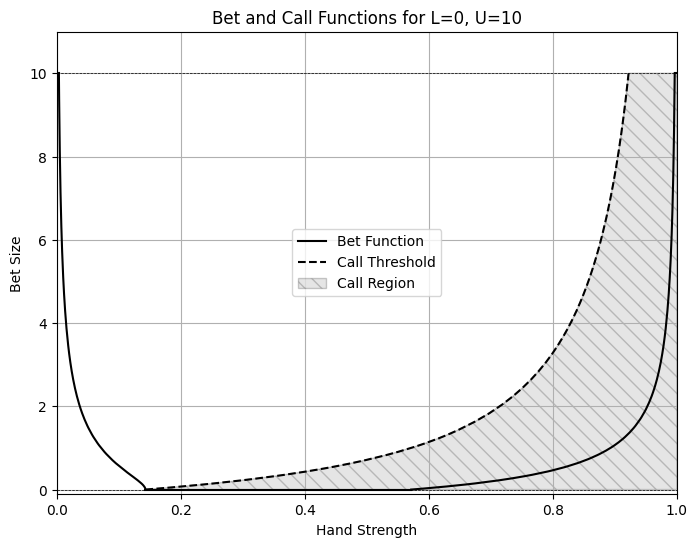
\includegraphics[width=\textwidth]{limit_continuous_0_10.png}
        \end{minipage}
        \hspace{0.05\textwidth}
        \begin{minipage}{0.6\textwidth}
            \centering
            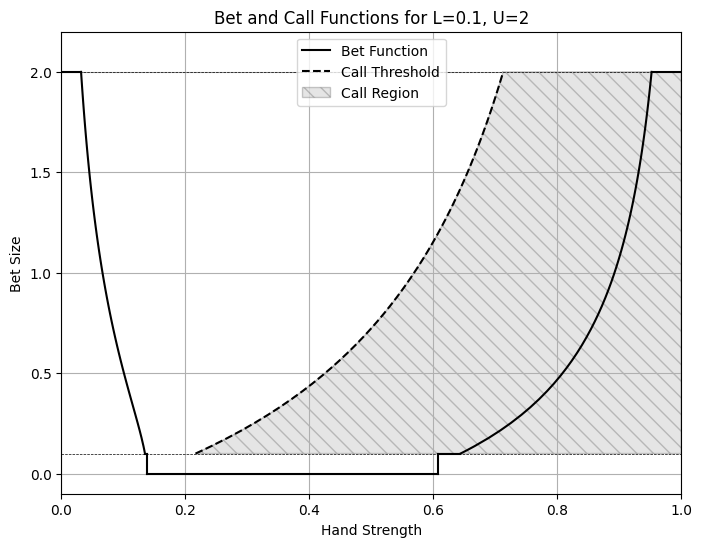
\includegraphics[width=\textwidth]{limit_continuous_0.1_2.png}
        \end{minipage}
        \vspace{0.5cm}\\
        \begin{minipage}{0.6\textwidth}
            \centering
            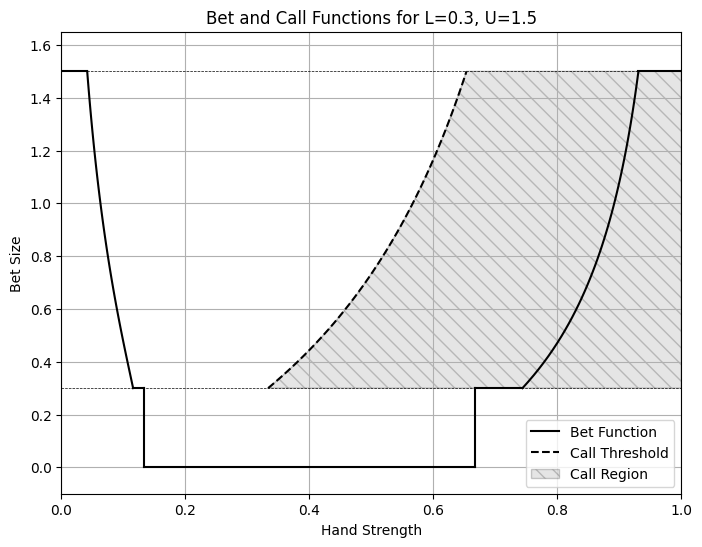
\includegraphics[width=\textwidth]{limit_continuous_0.3_1.5.png}
        \end{minipage}
        \hspace{0.05\textwidth}
        \begin{minipage}{0.6\textwidth}
            \centering
            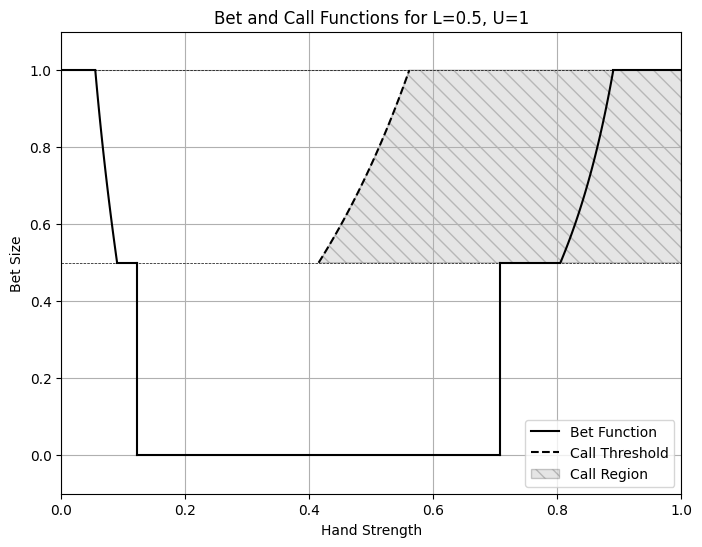
\includegraphics[width=\textwidth]{limit_continuous_0.5_1.png}
        \end{minipage}
    \end{adjustwidth}
    \caption{Nash equilibrium strategy profiles for different values of $L$ and $U$, from very lenient to very restricted bet sizes. The bet function maps hand strengths to bet sizes, while the call function gives the minimum calling hand strength for a given bet size. The shaded regions represent the hand strengths for which the caller should call a given bet size.}
    \label{fig:strategyprofile}
\end{figure}


\section{Game Value}
\label{sec:game_value}

We now consider the payoff to the bettor for possible hand combinations $x, y$ and the expected game value from a random hand combination. In Nash Equilibrium, a given hand combination $(x, y)$ uniquely determines the bettor's payoff, since both players play pure strategies. We can visualize the payoff for all hand combinations as a function defined on the unit square $[0, 1]^2$ (see Figure \ref{fig:gamevalue}).  

\begin{figure}[h!]
    \centering
    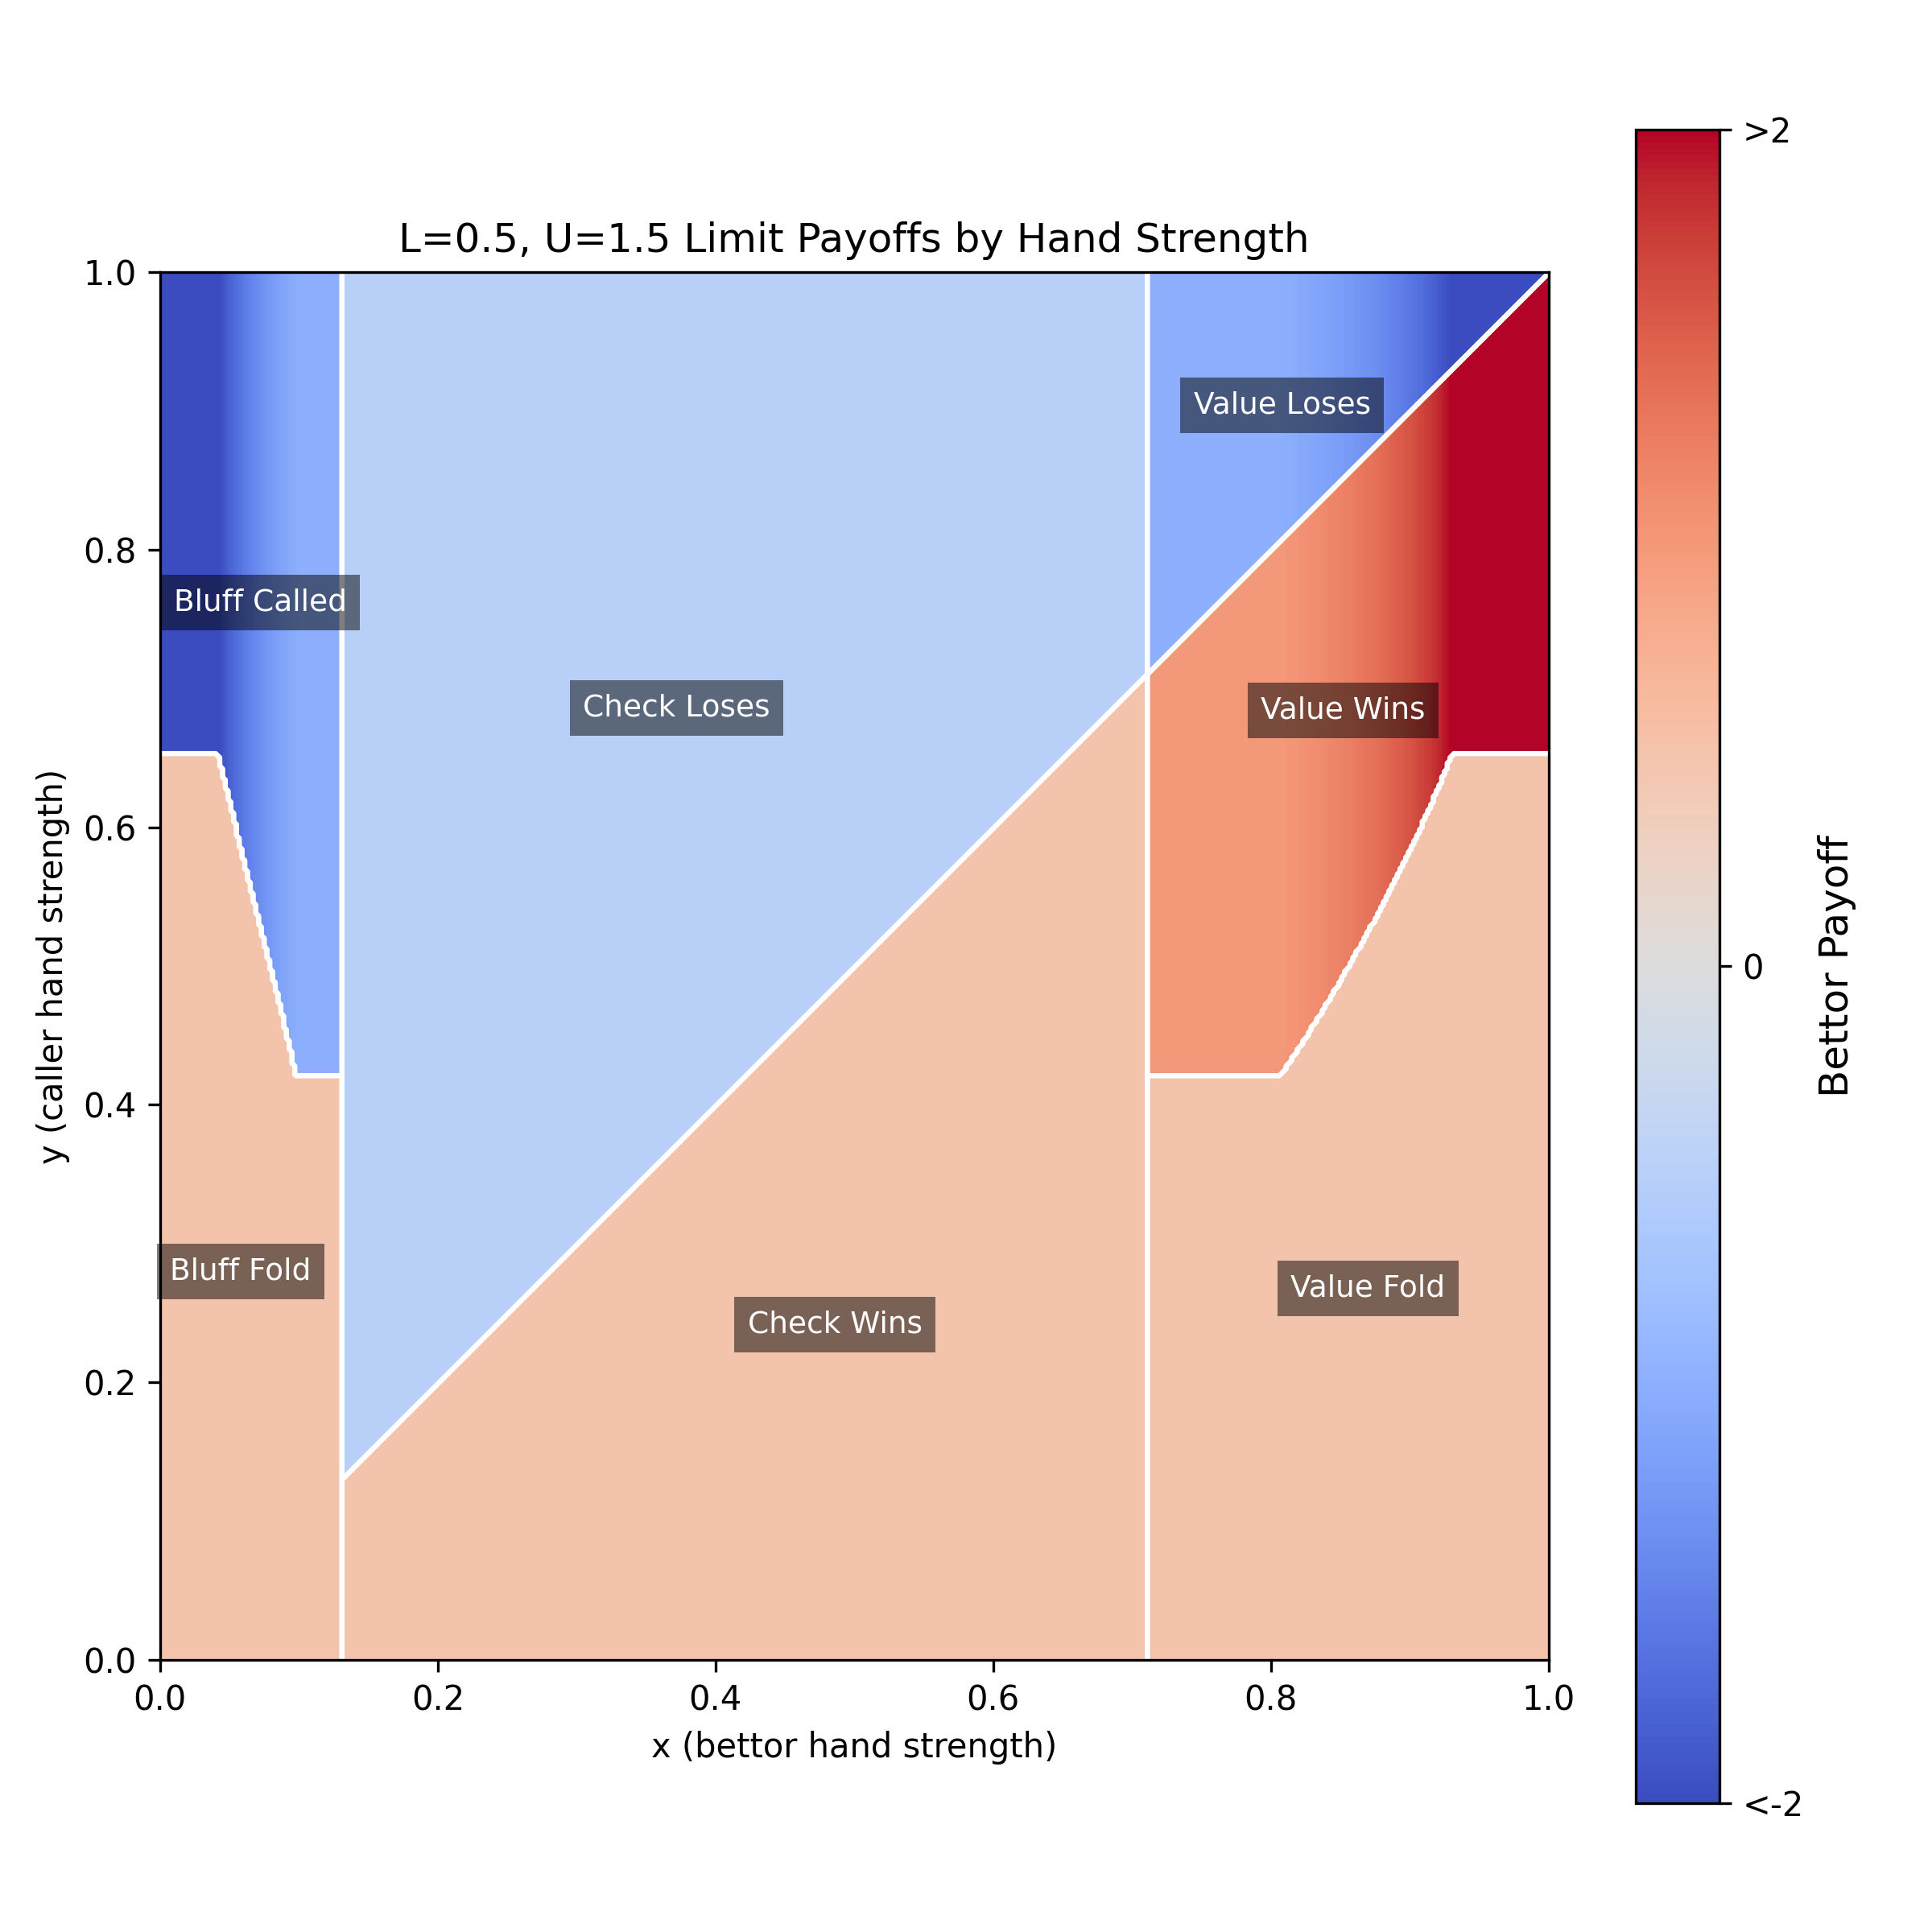
\includegraphics[width=0.7\textwidth]{LU_payoffs_0.5_1.5.png}
    \caption{Payoff to the bettor for all possible hand combinations $(x, y)$ in Limit Continuous Poker for $L=0.5, U=1.5$. The color scale represents the payoff to the bettor.}
    \label{fig:gamevalue}
\end{figure}

This gives insight into exactly how the bettor is gaining value from the game. In line with experience of real poker, the biggest wins and losses occur when both hands are strong (top right), with the stronger of the two hands winning a large pot. However, we also see large payoffs when a very weak bettor bluffs big and gets called by a strong caller (top left).  

The expected game value is the average of the payoff function over all possible hand combinations $(x, y)$, which can be computed as an integral of the payoff over the unit square. Because the bet size is only defined implicitly in terms of the hand strength $x$, this is extremely nontrivial and requires breaking the square into regions based on the strategies and bet size. This method is fully specified in the appendix, but the resulting expression is given below in terms of two subexpressions $V_{num}$ and $V_{den}$.

\begin{align*}
    V_{num}(L, U) =& L^6 \left(72 U^4+270 U^3+378 U^2+234 U+53\right) \\
        & -6 L^5 \left(3 U^6+42 U^5+87U^4+5 U^3-132 U^2-123 U-33\right)\\
        & -3 L^4 \left(3 U^6+258 U^5+825 U^4+862 U^3+171U^2-216 U-90\right) \\ 
        &-2 L^3 \left(-72 U^6+288 U^5+1620 U^4+2321 U^3+1203 U^2+51U-81\right) \\
        & +3 L^2 \left(97 U^6+102 U^5-465 U^4-1020 U^3-705 U^2-138 U+12\right) \\
        & +6 LU \left(35 U^5+90 U^4+27 U^3-108 U^2-111 U-30\right) \\ 
        & +U \left(53 U^5+174 U^4+183U^3+36 U^2-45 U-18\right)\\
    V_{den}(L, U) =& L^3 \left(6 U^3+18 U^2+18 U+5\right)\\
        &+3 L^2\left(7 U^3+21 U^2+21 U+6\right)\\
        &+3 L \left(7 U^3+21 U^2+21 U+6\right)\\
        &+7 U^3+21U^2+21 U+6 \\
    V_{LCP}(L, U) =& \frac{-V_{num}(L, U)}{2 V_{den}(L, U)^2}\\
\end{align*}

This does turn out to be a rational function of $L$ and $U$. Importantly, this makes it easy to compute $V_{LCP}(L, U)$ as $L, U$ approach their extreme values, which we use to relate the game value to that of NLCP and FBCP in section \ref{sec:game_value_convergence}.

\section{Interpretation}
The most natural way to think of Limit Continuous Poker is as a generalization between Fixed-Bet and No-Limit Continuous Poker, on a spectrum from strict to lenient bet sizing. It is helpful to think in this context when interpreting the strategies and game value. In this light, we begin by asking whether the Nash equilibrium strategies approach those of NLCP and FCP as the limits $L$ and $U$ approach their extreme cases. To make this more explicit, we model the bettor strategies for all three games as `bet functions’ from hand strengths to bets (with 0 representing a check), and caller strategies as `call functions’ from bet sizes to minimum calling thresholds. We also introduce notation to reference all three strategy profiles more efficiently.

\subsection{Notation}

Let $S_B(x)$ denote the bet function for fixed bet size $B$ in Continuous Poker, which maps hand strenths $x$ to bets (either $0$ for a check of $B$ for a bet). Let $C_B(s)$ denote the call function which maps the set of bets (the singleton set $\{B\}$) to calling thresholds. 

\begin{align}
	S_B(x) & = \begin{cases}
    B & x < \frac{B}{(1+2B)(2+B)}\\
    0 & \frac{B}{(1+2B)(2+B)} > x > \frac{1 + 4B + 2B^2}{(1+2B)(2+B)}\\
    B & x > \frac{1 + 4B + 2B^2}{(1+2B)(2+B)}
\end{cases} \\
C_B(s) & = \frac{B(3 +2B)}{(1+2B)(2+B)}
\end{align}

Let $S(x)$ denote the bet function for NLCP, which maps hand strengths $x$ to bet sizes $s > 0$. Let $C(s)$ denote the call function which maps the set of bets (the interval $[0, \infty)$) to calling thresholds. $S(x)$ is harder to define explicitly because the bettor strategy for NLCP is defined by functions $v(s)$ and $b(s)$ which map bet sizes to hand strengths, and $S(x)$ is related to the inverse functions $v^{-1}(x)$ and $b^{-1}(x)$. 

Finally, let $S_L^U(x)$ and $C_L^U(s)$ denote the bet and call functions for Limit Continuous Poker, which map hand strengths $x$ to bet sizes $s \in [L, U]$ and bet sizes $s \in [L, U]$ to calling thresholds. Like $S(x)$, $S_L^U(x)$ will be a piecewise function with some parts being defined by the inverse functions $v^{-1}(x)$ and $b^{-1}(x)$. We also adapt this notation to the $x_i$'s in the solution so that $x_i|_a^b$ means $x_i$ with $L=a$ and $U=b$.

To compare the three strategy profiles, we want to know whether the bet and call functions for Limit Continuous Poker approach those of Continuous Poker and NLCP as the limits $L$ and $U$ approach their extreme values.

\subsection{Strategic Convergence}
\label{sec:strategic_convergence}

\subsubsection{Bettor Strategy Convergence to Continuous Poker}
We expect that as $L$ and $U$ approach some fixed value $s$, the bet function $S_L^U(x)$ should converge to the bet function $S_B(x)$ for Continuous Poker with a fixed bet size $B$. 

\begin{theorem}
	 For any $B > 0$, the bet function $S_L^U(x)$ for Limit Continuous Poker converges to the bet function $S_B(x)$ for Continuous Poker with a fixed bet size $B$ as $L$ and $U$ approach $B$:
\[
\lim_{L \to B} \lim_{U \to B} S_L^U(x) = \lim_{U \to B} \lim_{L \to B} S_L^U(x) = S_B(x).
\]
\end{theorem}

\begin{customproof}
We analyze the expressions for the $x_i$'s, each of which is a rational function of $L$ and $U$ (i.e., a ratio of polynomials in $L$ and $U$). Since these functions are well-defined for all positive values of $L$ and $U$, the limit as $L \to s$ and $U \to s$ is well-behaved. By substituting $L = U = B$ for some fixed $B$, we obtain the following:

\begin{align*}
    x_0|_B^B & = x_1|_B^B = \frac{B}{2 B^3+7 B^2+7 B+2} \\
    x_2|_B^B & = \frac{B}{(1+2B)(2+B)} \\
    x_3|_B^B & = \frac{2 B^2+4 B+1}{(1+2B)(2+B)} \\
    x_4|_B^B & = x_5|_B^B = \frac{2 B^2+5 B+1}{(1+2B)(2+B)} \\
\end{align*}

$x_0 = x_1$ and $x_4 = x_5$ are expected, since these intervals are where the bettor uses an intermediate bet size, and $L=U=B$ does not allow intermediate bet sizes. This reduces the bet function to 

\begin{align*}
    \lim_{L \to B} \lim_{U \to B} S_L^U(x) & = \begin{cases}
    B & x < \frac{B}{(1+2B)(2+B)}\\
    0 & \frac{B}{(1+2B)(2+B)} > x > \frac{2 B^2+4 B+1}{(1+2B)(2+B)}\\
    B & x > \frac{2 B^2+4 B+1}{(1+2B)(2+B)}
    \end{cases}\\
    &= S_B(x)
\end{align*}
\end{customproof}

\subsubsection{Caller Strategy Convergence to Continuous Poker}

The calling function is easier to analyze. We want to show that the calling threshold $C_L^U(s)$ converges to the calling threshold $C_B(s)$ for Continuous Poker with a fixed bet size $B$ as $L$ and $U$ approach $B$.

\begin{theorem}
     For any $B > 0$, the call function $C_L^U(s)$ for Limit Continuous Poker converges to the call function $C_B(s)$ for Continuous Poker with a fixed bet size $B$ as $L$ and $U$ approach $B$:
\[
\lim_{L \to B} \lim_{U \to B} C_L^U(s) = \lim_{U \to B} \lim_{L \to B} C_L^U(s) = C_B(s).
\]
\end{theorem}

\begin{customproof}
We already have the value of $x_2|_B^B$, so we can plug this into the expression for the calling threshold:
\begin{align*}
    \lim_{L \to B} \lim_{U \to B} C_L^U(s) & = \lim_{L \to B} \lim_{U \to B} \frac{x_2+B}{1+B} \\
    & = \frac{\frac{B}{(1+2B)(2+B)} + B}{1+B} \\
    & = \frac{B(3+2B)}{(1+2B)(2+B)} \\
    & = C_B(s)
\end{align*}
\end{customproof}

\subsubsection{Bettor Strategy Convergence to NLCP}

In a similar fashion, we expect that as $L$ and $U$ approach $0$ and $\infty$, the bet function $S_L^U(x)$ should converge to the bet function $S(x)$ for NLCP.

\begin{theorem}
    The bet function $S_L^U(x)$ for Limit Continuous Poker converges to the bet function $S(x)$ for NLCP as $L$ and $U$ approach $0$ and $\infty$:
\[
\lim_{L \to 0} \lim_{U \to \infty} S_L^U(x) = \lim_{U \to \infty} \lim_{L \to 0} S_L^U(x) = S(x).
\]
\end{theorem}
\begin{customproof}
We can analyze the expressions for the $x_i$'s as $L$ and $U$ approach $0$ and $\infty$. The limit is well-defined, and we can substitute $L=0$ and $U=\infty$ into the expressions for the $x_i$s.
\begin{align*}
    x_0|_0^\infty &= 0 \\
    x_1|_0^\infty &= x_2|_0^\infty = \frac{1}{7} \\
    x_3|_0^\infty &= x_4|_0^\infty = \frac{4}{7} \\
    x_5|_0^\infty &= 1
\end{align*}

$x_0|_0^\infty = 0$ and $x_5|_0^\infty = 1$ are expected, since these intervals are where the bettor uses a minimum bet size and a maximum bet size, respectively, both of which are impossible. The bettor now bets intermediate values for $x < \frac{1}{7}$ and $x > \frac{4}{7}$, and checks for $\frac{1}{7} < x < \frac{4}{7}$. But how much do they bet? We can take the limits of $v(s)$ and $b(s)$ as $L$ and $U$ approach $0$ and $\infty$:

\begin{align*}
    \lim_{L \to 0} \lim_{U \to \infty} b(s) &= \frac{3 s+1}{7 (s+1)^3}\\
    \lim_{L \to 0} \lim_{U \to \infty} v(s) &= 1 - \frac{3}{7 (s+1)^2}
\end{align*}

To summarize, the bettor bets $s$ with hands $x < \frac{1}{7}$ such that $x = b(s)$ or hands $x > \frac{4}{7}$ such that $x = v(s)$. This is exactly the same as the bet function for NLCP described in section \todo{ref}.

\end{customproof}

\subsubsection{Caller Strategy Convergence to NLCP}

The calling function is again easier to analyze. We want to show that the calling threshold $C_L^U(s)$ converges to the calling threshold $C(s)$ for NLCP as $L$ and $U$ approach $0$ and $\infty$.
\begin{theorem}
    The call function $C_L^U(s)$ for Limit Continuous Poker converges to the call function $C(s)$ for NLCP as $L$ and $U$ approach $0$ and $\infty$:
\[
\lim_{L \to 0} \lim_{U \to \infty} C_L^U(s) = \lim_{U \to \infty} \lim_{L \to 0} C_L^U(s) = C(s).
\]
\end{theorem}
\begin{customproof}
Again, we already have the limiting value of $x_2|_0^\infty$, so we can plug this into the expression for the calling threshold:
\begin{align*}
    \lim_{L \to 0} \lim_{U \to \infty} C_L^U(s) & = \lim_{L \to 0} \lim_{U \to \infty} \frac{x_2+s}{1+s}\\
    & = \frac{\frac{1}{7}+s}{1+s}\\
    & = 1 - \frac{6}{7(1+s)}\\
    & = C(s)
\end{align*}
\end{customproof}

% v(s)=x
% v_inv(x)=s
% y > c(v_inv(x))
% c_inv(y) > v_inv(x)
% v(c_inv(y)) > x to call

\subsection{Game Value Convergence}
\label{sec:game_value_convergence}

Recall that FBCP and NLCP have values

\begin{align*}
    V_{FB}(B) &= \frac{B}{2(1+2B)(2+B)} \\
    V_{NL} & = \frac{1}{14}
\end{align*}

The value of LCP is given in section \ref{sec:game_value}. A common theme throughout our previous analysis has been treating Limit Continuous Poker as a generalization between Fixed-Bet and No-Limit. The value of the games follows this theme as well.

To see this visually, we can look at the expected value of the game as a function of the limits $L$ and $U$ in Figure \ref{fig:payoffs_vs_LU_combined}.

\begin{figure}[h!]
    \begin{adjustwidth}{-1in}{-1in}
        \centering
        \begin{minipage}{0.6\textwidth}
            \centering
            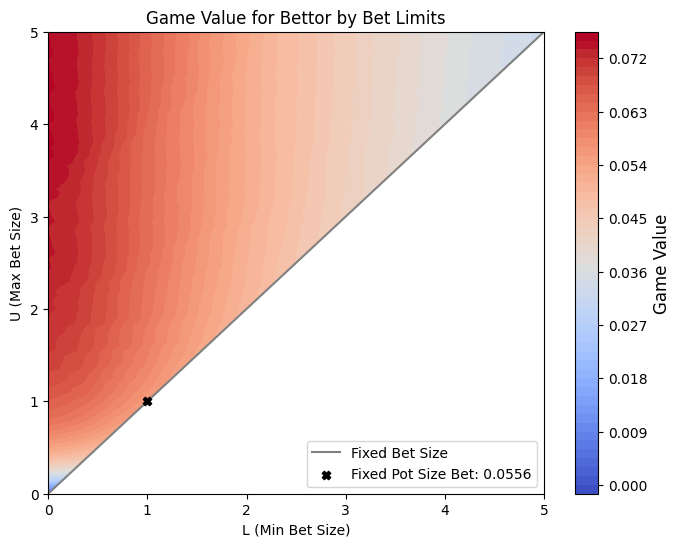
\includegraphics[width=\textwidth]{value_by_LU.png}
            \caption*{(a) Linear scale}
        \end{minipage}
        \hspace{0.05\textwidth}
        \begin{minipage}{0.6\textwidth}
            \centering
            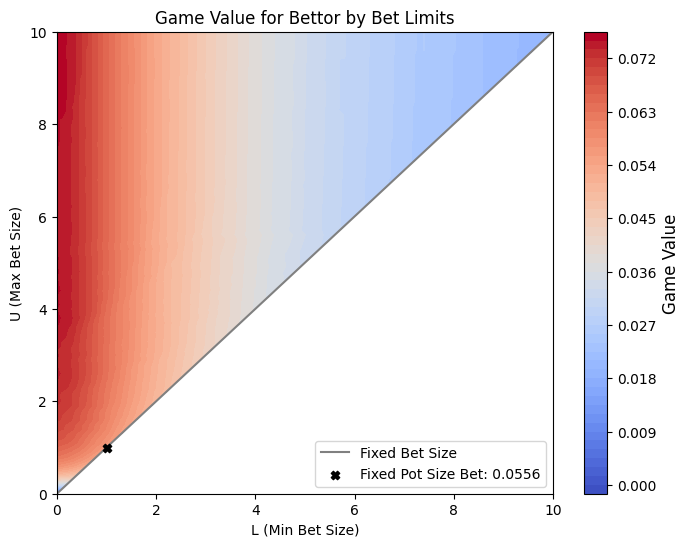
\includegraphics[width=\textwidth]{value_LU_wide.png}
            \caption*{(b) Zoomed out linear scale}
        \end{minipage}
        \vspace{0.5cm}
        \begin{minipage}{0.6\textwidth}
            \centering
            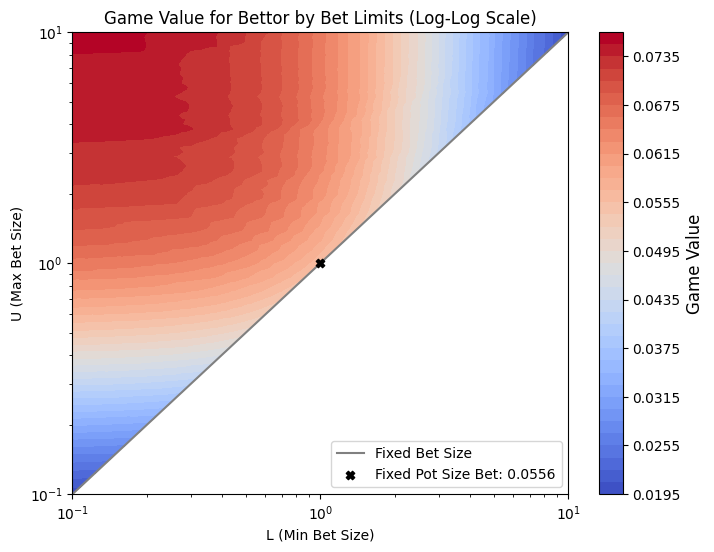
\includegraphics[width=\textwidth]{value_LU_log.png}
            \caption*{(c) Log-log scale}
        \end{minipage}
        \hspace{0.05\textwidth}
        \begin{minipage}{0.6\textwidth}
            \centering
            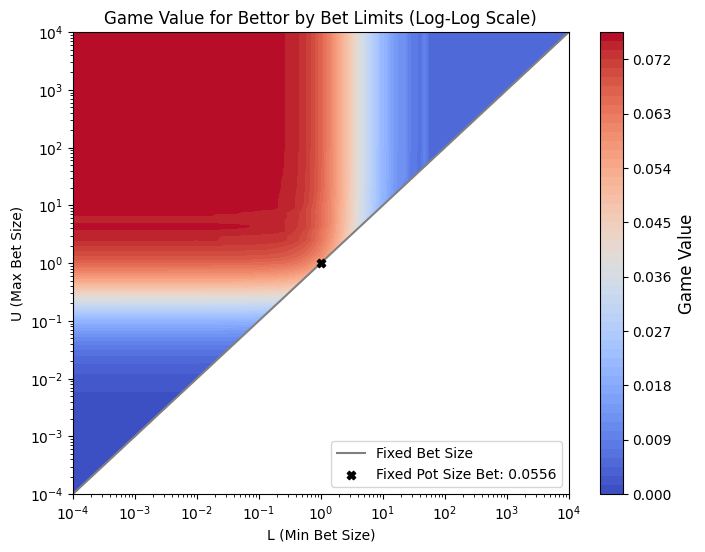
\includegraphics[width=\textwidth]{value_LU_log_big.png}
            \caption*{(d) Zoomed out log-log scale}
        \end{minipage}
    \end{adjustwidth}
    \caption{Game value of Limit Continuous Poker as a function of the limits $L$ and $U$. (a) Linear scale, (b) Zoomed out linear scale, (c) Log-log scale, (d) Zoomed out log-log scale. The restriction $L \leq U$ keeps the plots above the diagonal.}
    \label{fig:payoffs_vs_LU_combined}
\end{figure}

Intuitively, more options for the bettor should increase the game's value, and we see that reflected by higher value for more lenient limits (top left of any plot in Figure \ref{fig:payoffs_vs_LU_combined}) and lower value for more strict limits (moving down/right). These plots also align with the known result that a fixed pot-size bet of $B=1$ maximizes the expected value for the bettor in FBCP, as seen by the fact that $(1, 1)$ achieves the maximum value on the diagonal. 

However, it remains to be proven that the value of Limit Continuous Poker actually converges to the value of FBCP as $L$ and $U$ approach some fixed value $B$.

\begin{theorem}
    For any $B > 0$, the value of Limit Continuous Poker converges to the value of Fixed-Bet Continuous Poker as $L$ and $U$ approach $B$:
\[
\lim_{L \to B} \lim_{U \to B} V_{LCP}(L, U) = \lim_{U \to B} \lim_{L \to B} V_{LCP}(L, U) = V_{FB}(B)
\]
\end{theorem}

What happens to the game value as $U$ and $L$ approach extremes $0$ and $\infty$? Zooming out reveals that as $U$ becomes very large compared to the pot of 1, further increasing $U$ has diminishing returns on the game value (in plot (b), horizontal strips near the top edge become indistinguishable). This remains true even on a log-log plot, indicating that even increasing $U$ exponentially does not increase the game value meaningfully. The same can be said as $L$ approaches $0$. This observation leads us to the following theorem:

\begin{theorem}
    The value of Limit Continuous Poker converges to the value of NLCP as $L$ and $U$ approach $0$ and $\infty$:
\[
\lim_{L \to 0} \lim_{U \to \infty} V_{LCP}(L, U) = \lim_{U \to \infty} \lim_{L \to 0} V_{LCP}(L, U) = V_{NL}
\]
\end{theorem}

However, this should not be surprising given that NLCP has a finite value. If, as we reasoned above, more options for the bettor monotonically increase the game value, then the game value must be bounded above by the value of NLCP, where the bettor's choice is maximized. Indeed, plot (d) seems to show that the game value approaches a finite supremum ($\approx 0.072\approx 1/14$) even as $L$ and $U$ approach their extremes (top left of the plot).  

This can be broken down further by consider the combinations of hand strengths which result in certain payoffs in Nash equilibrium, as in section \todo{ref}. Figure \ref{fig:payoffs} shows the payoffs as a function of hand strengths $x$ and $y$ for various values of $L, U$. 


\begin{figure}[h!]
    \begin{adjustwidth}{-1in}{-1in}
        % \vspace{-3cm} % Move the figure up into the top margin
        \centering
        \begin{minipage}{0.4\textwidth}
            \centering
            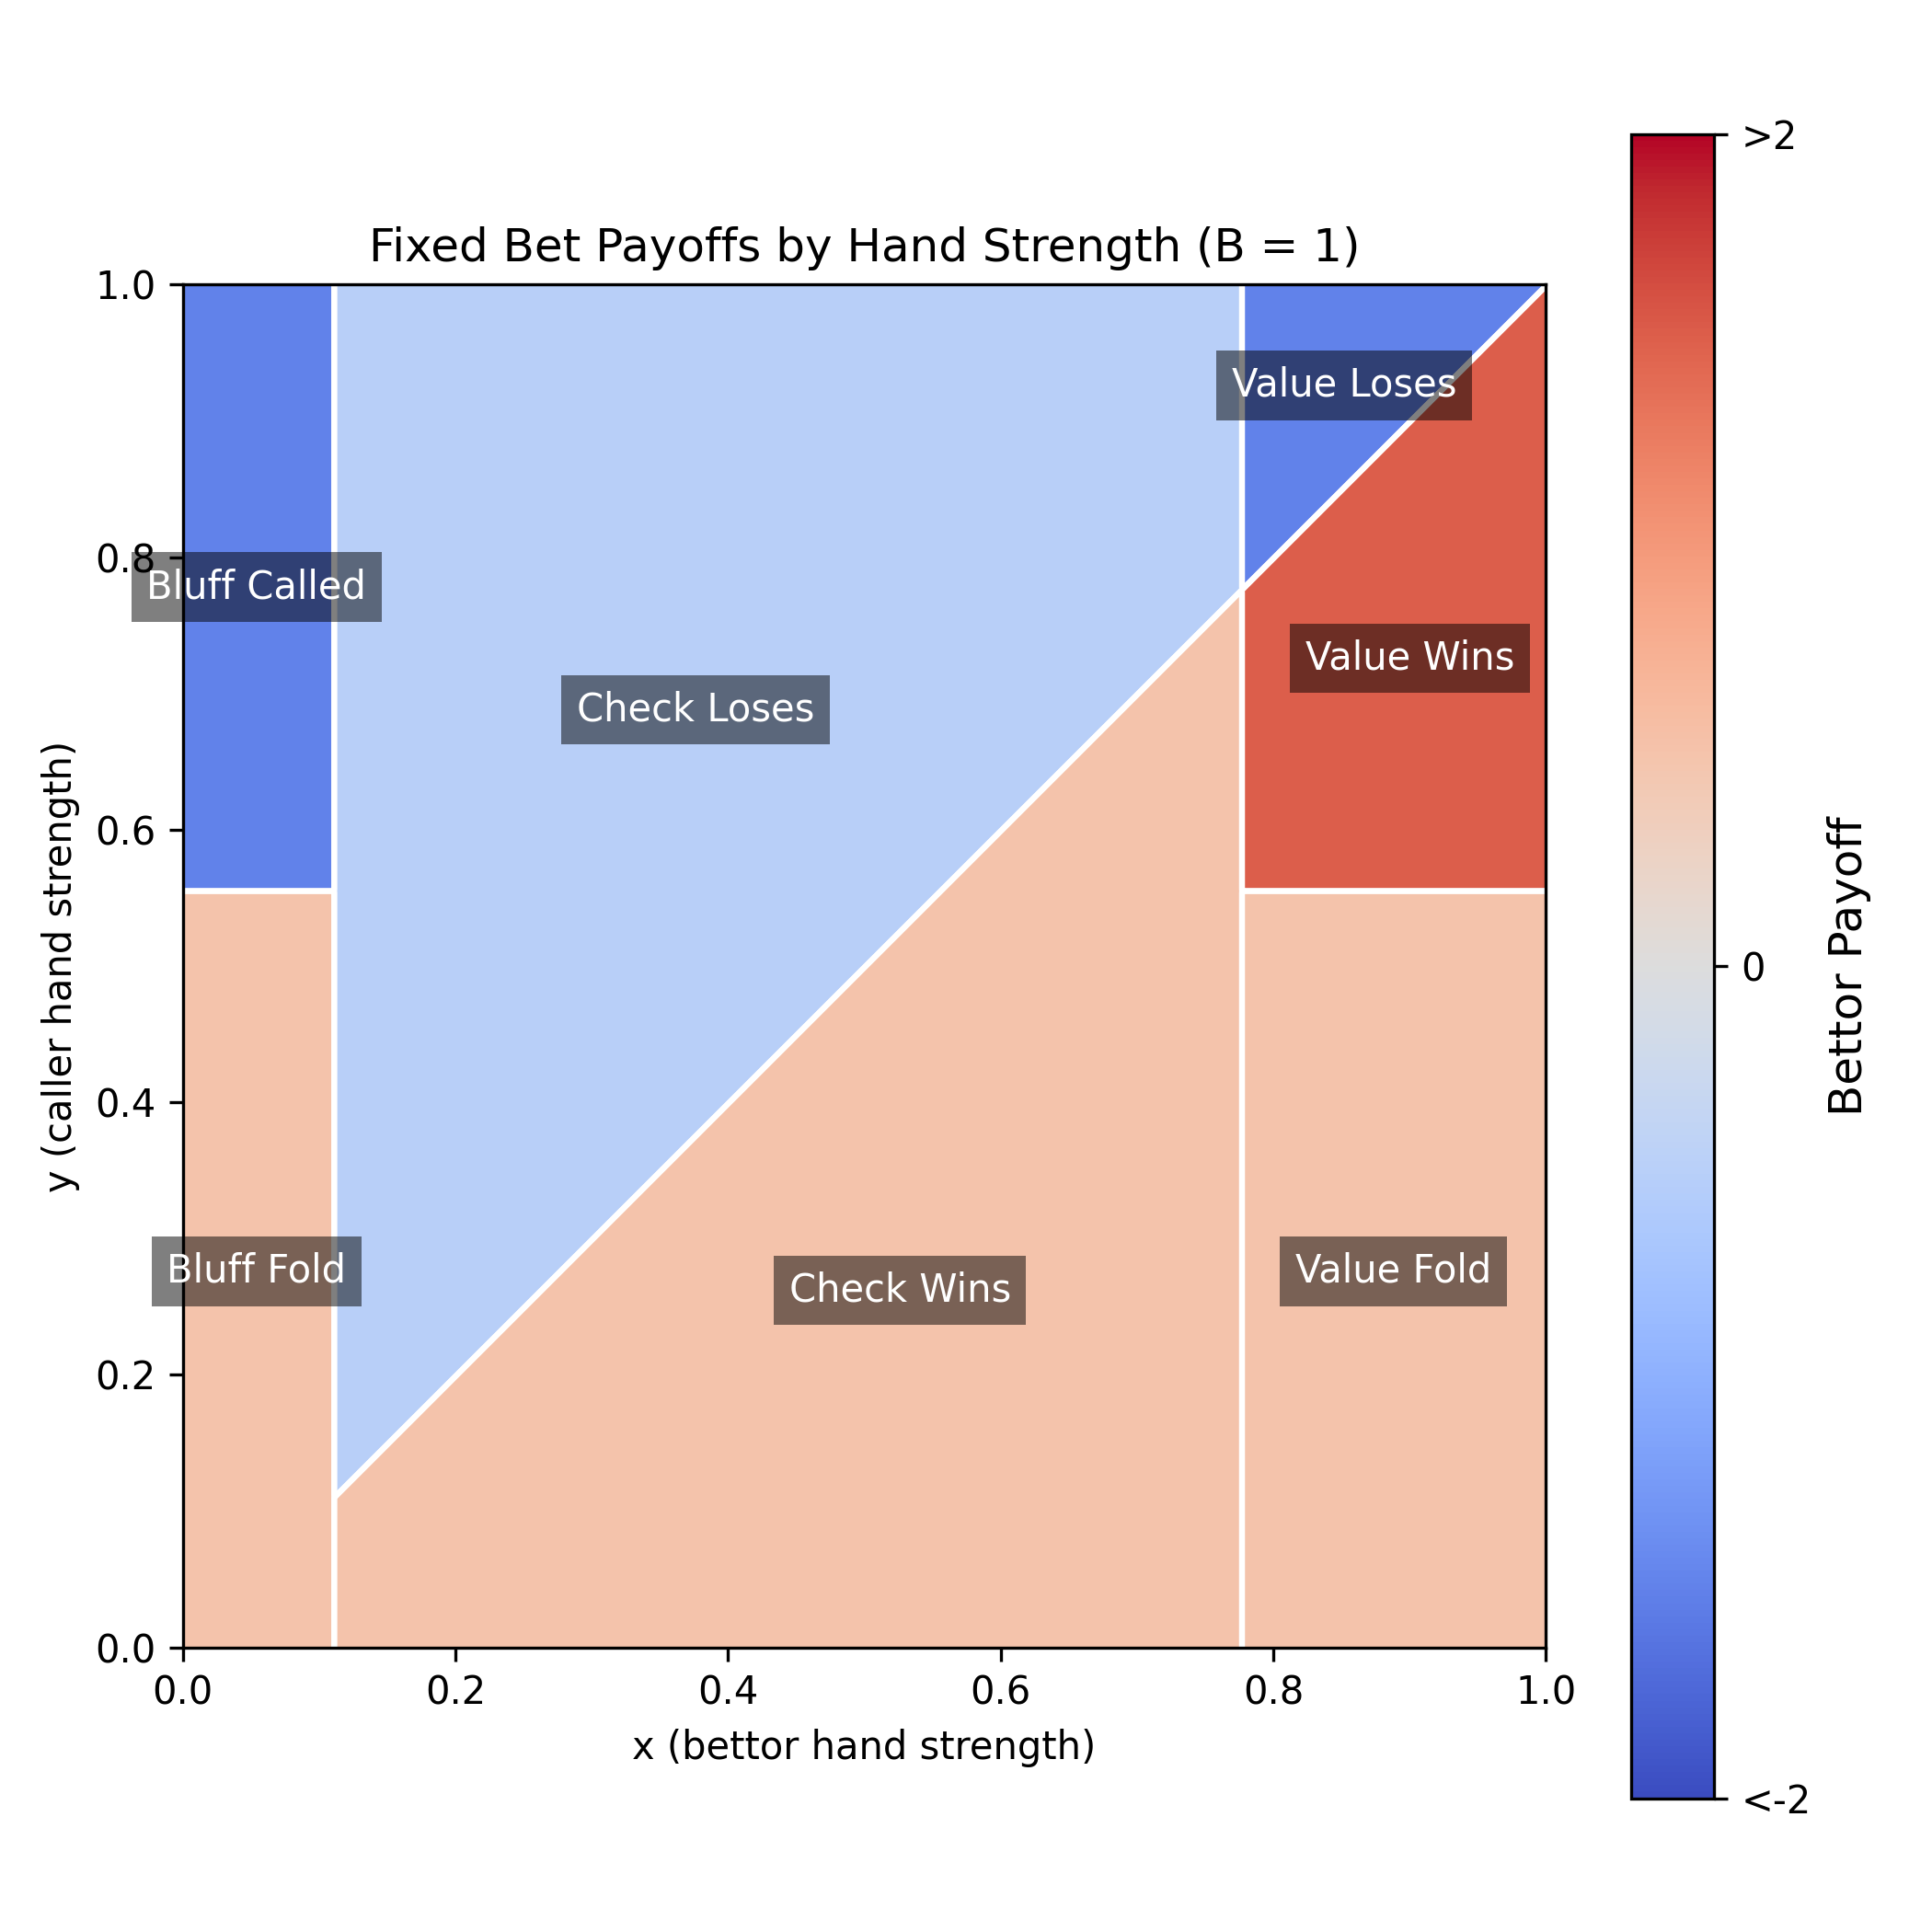
\includegraphics[width=\textwidth]{payoff_fixed_bet_heatmap.png}
        \end{minipage}
        \hspace{0.02\textwidth}
        \begin{minipage}{0.4\textwidth}
            \centering
            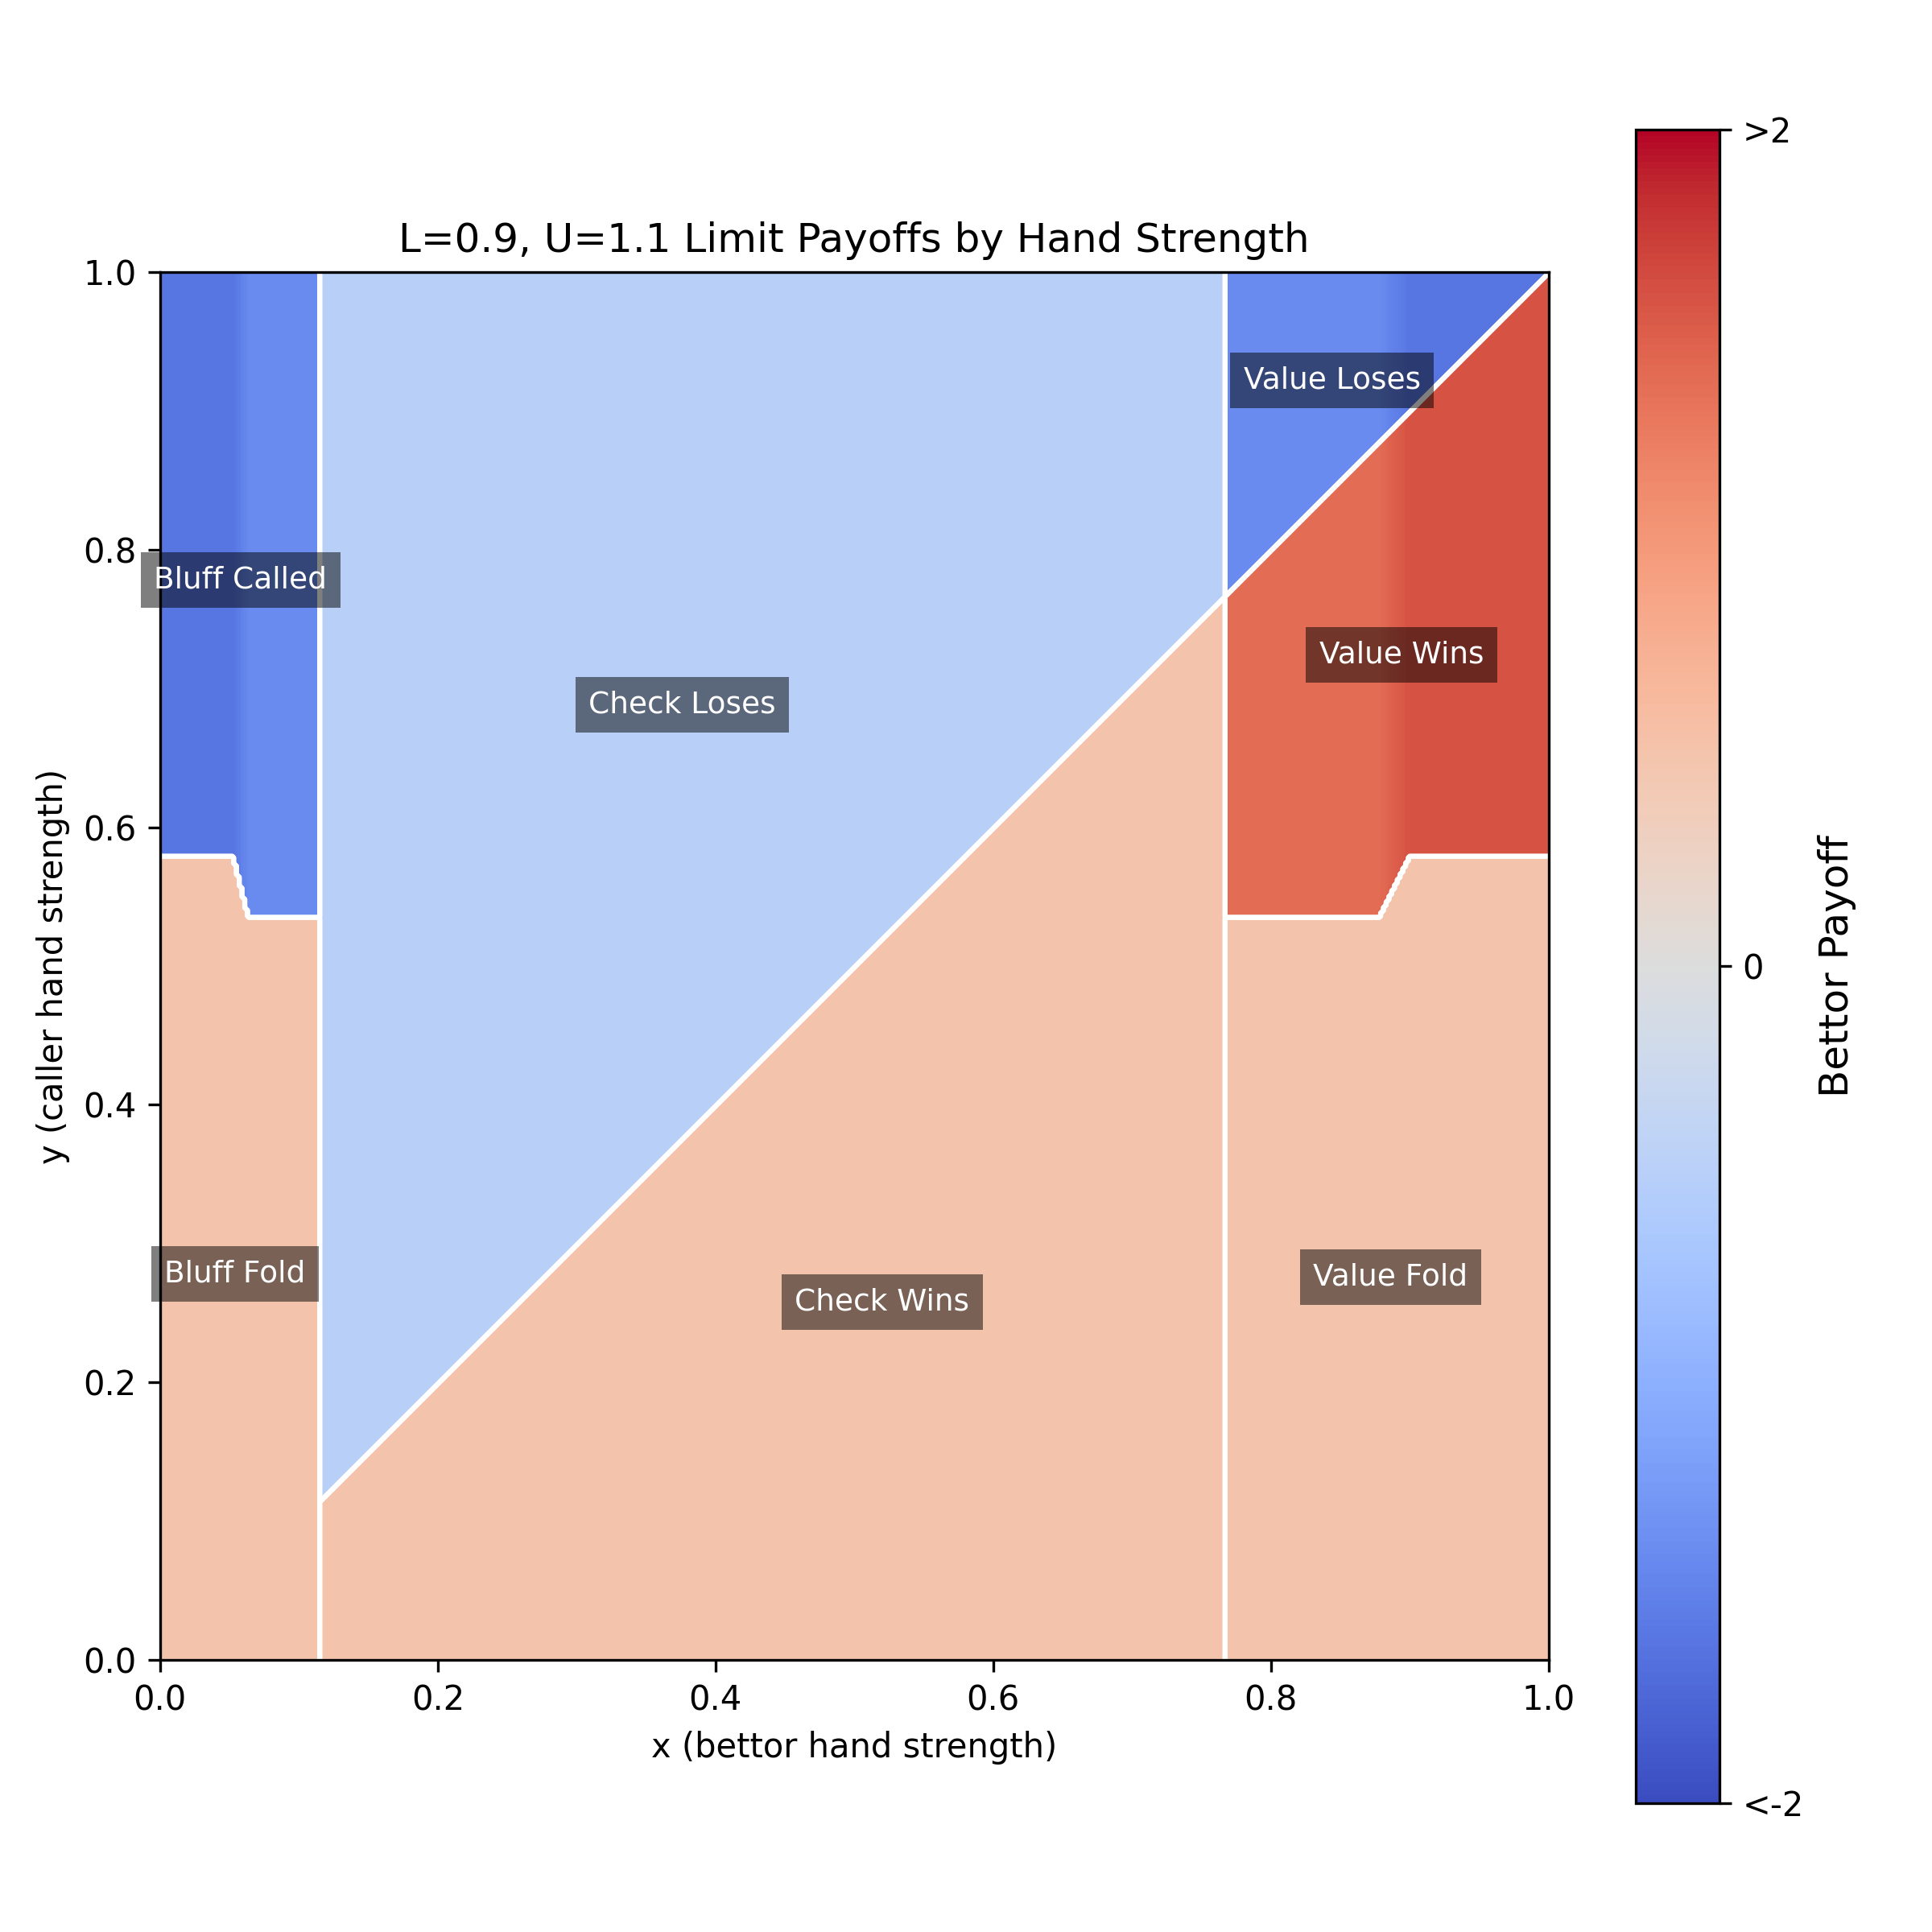
\includegraphics[width=\textwidth]{LU_payoffs_0.9_1.1.png}
        \end{minipage}
        \hspace{0.02\textwidth}
        \begin{minipage}{0.4\textwidth}
            \centering
            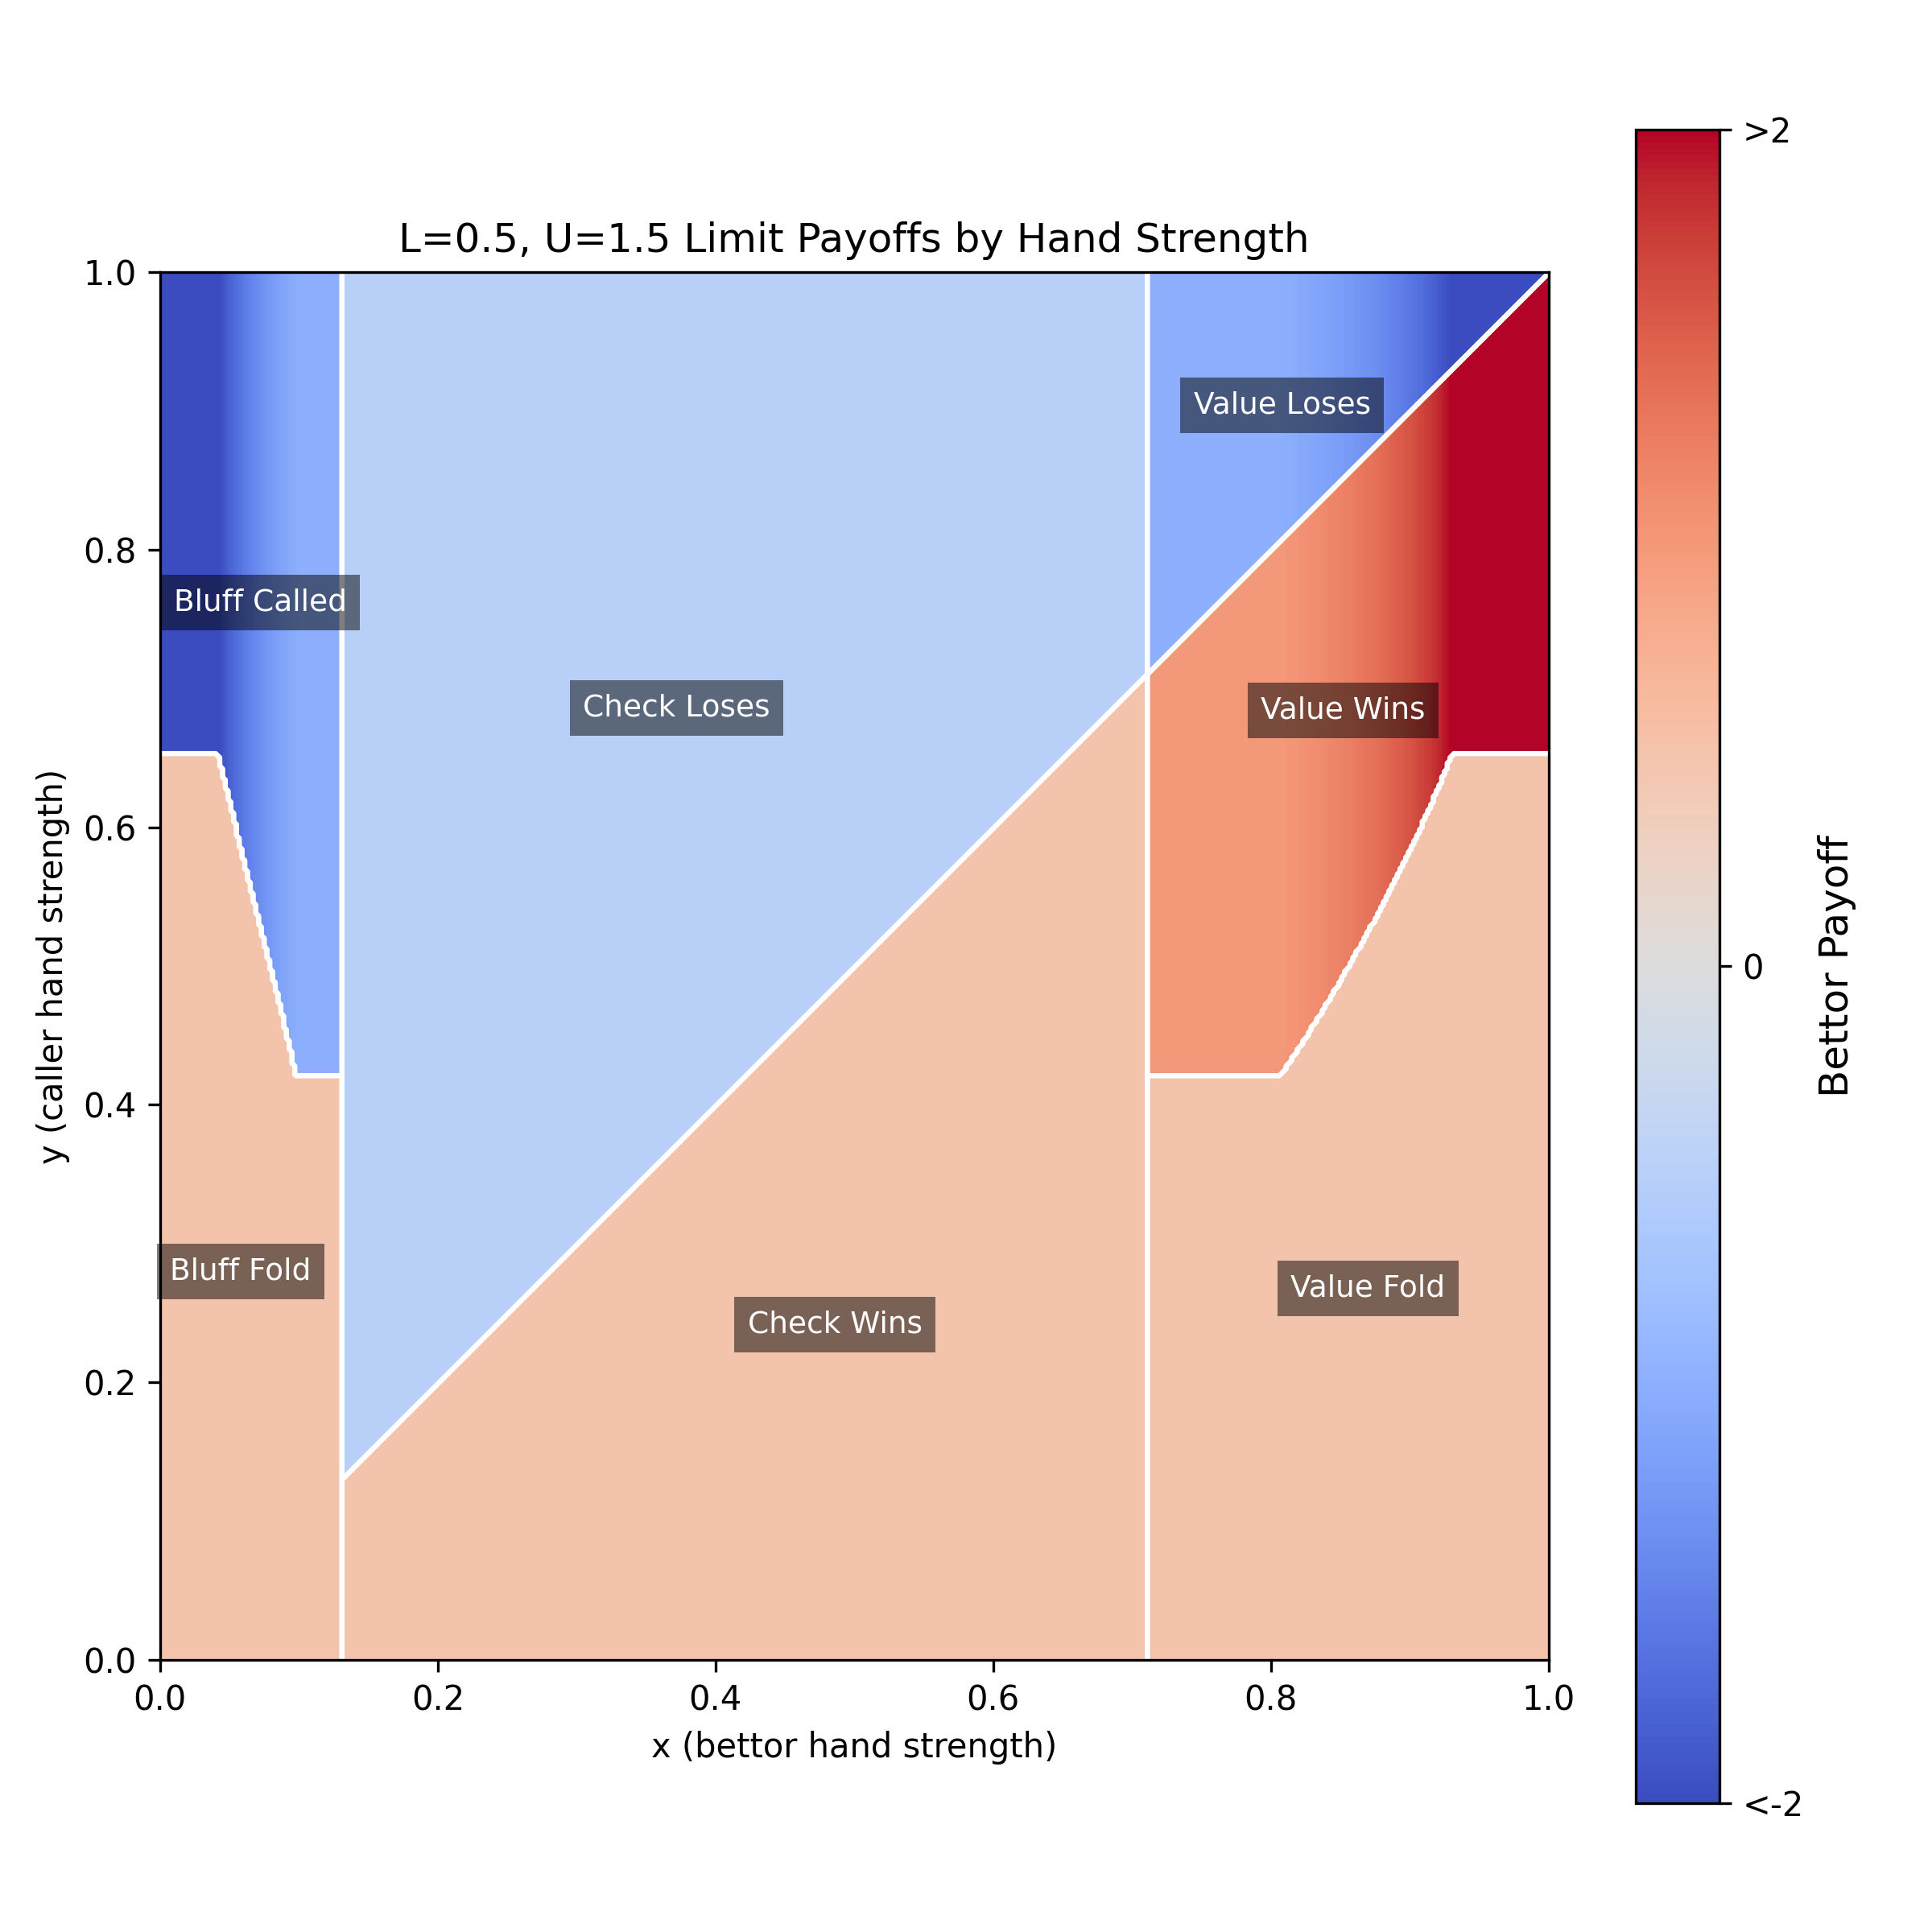
\includegraphics[width=\textwidth]{LU_payoffs_0.5_1.5.png}
        \end{minipage}
        \vspace{-0.5cm}\\ % Reduced vertical space
        \begin{minipage}{0.4\textwidth}
            \centering
            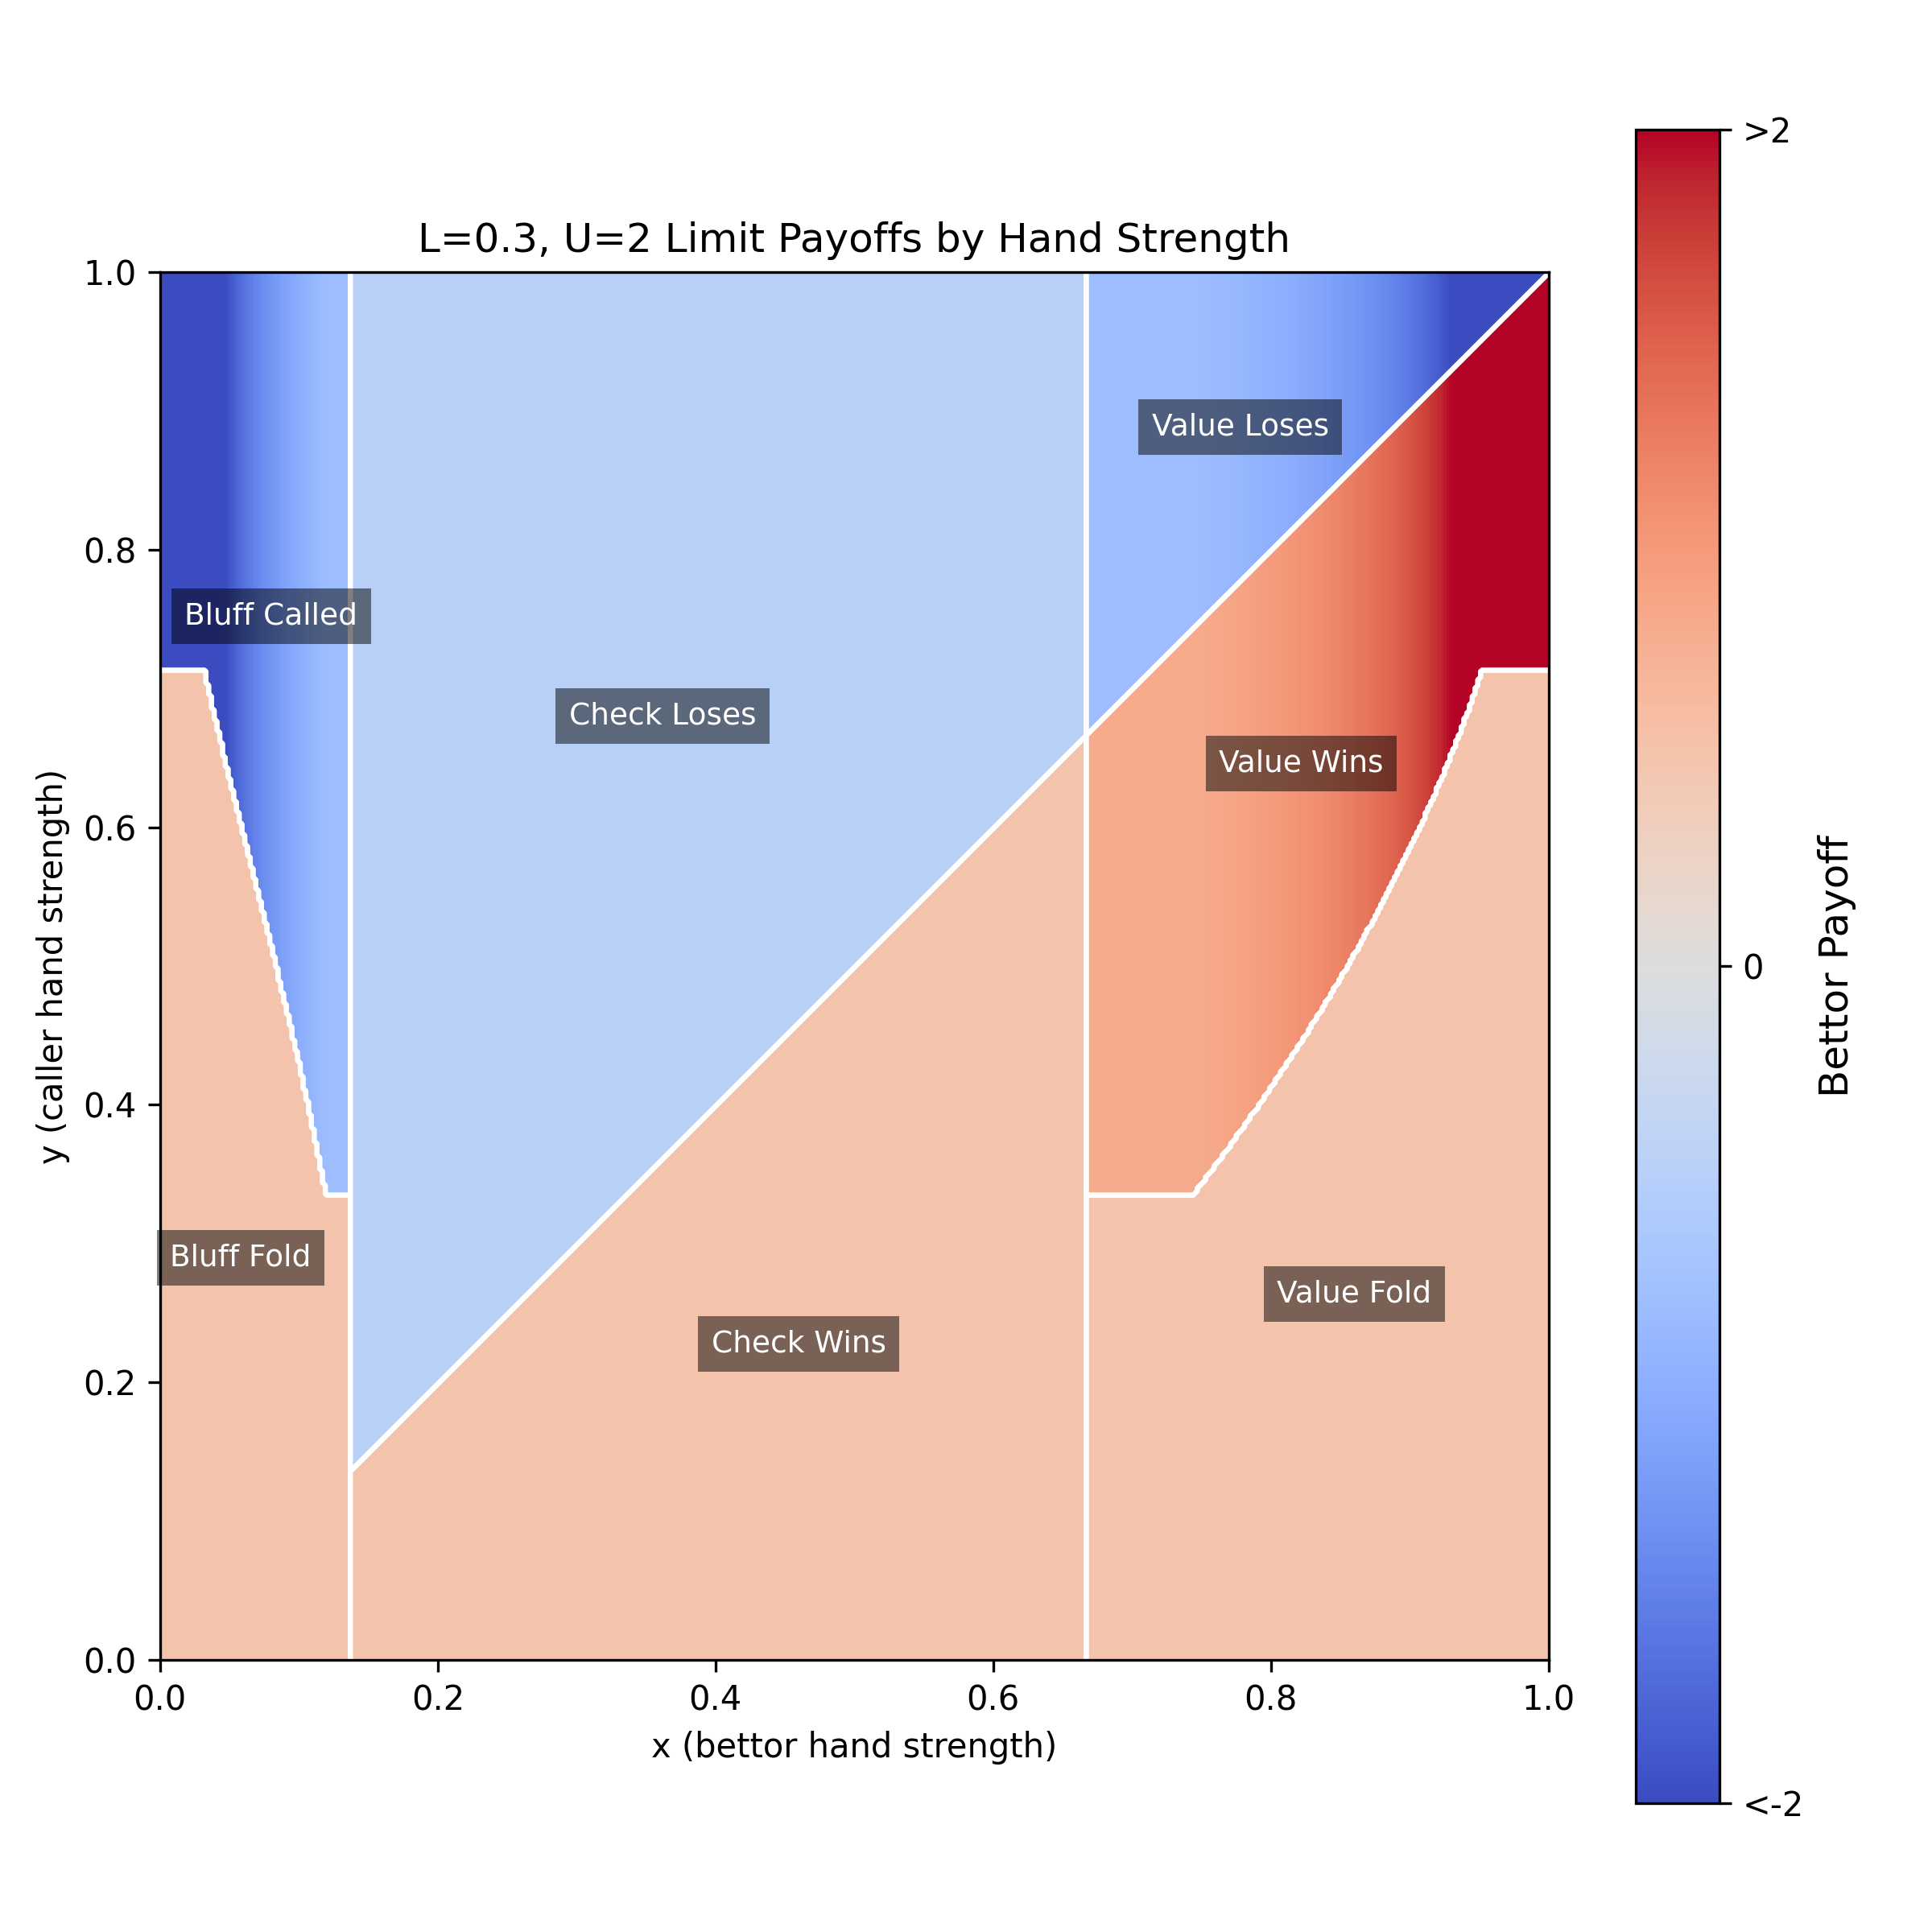
\includegraphics[width=\textwidth]{LU_payoffs_0.3_2.png}
        \end{minipage}
        \hspace{0.02\textwidth}
        \begin{minipage}{0.4\textwidth}
            \centering
            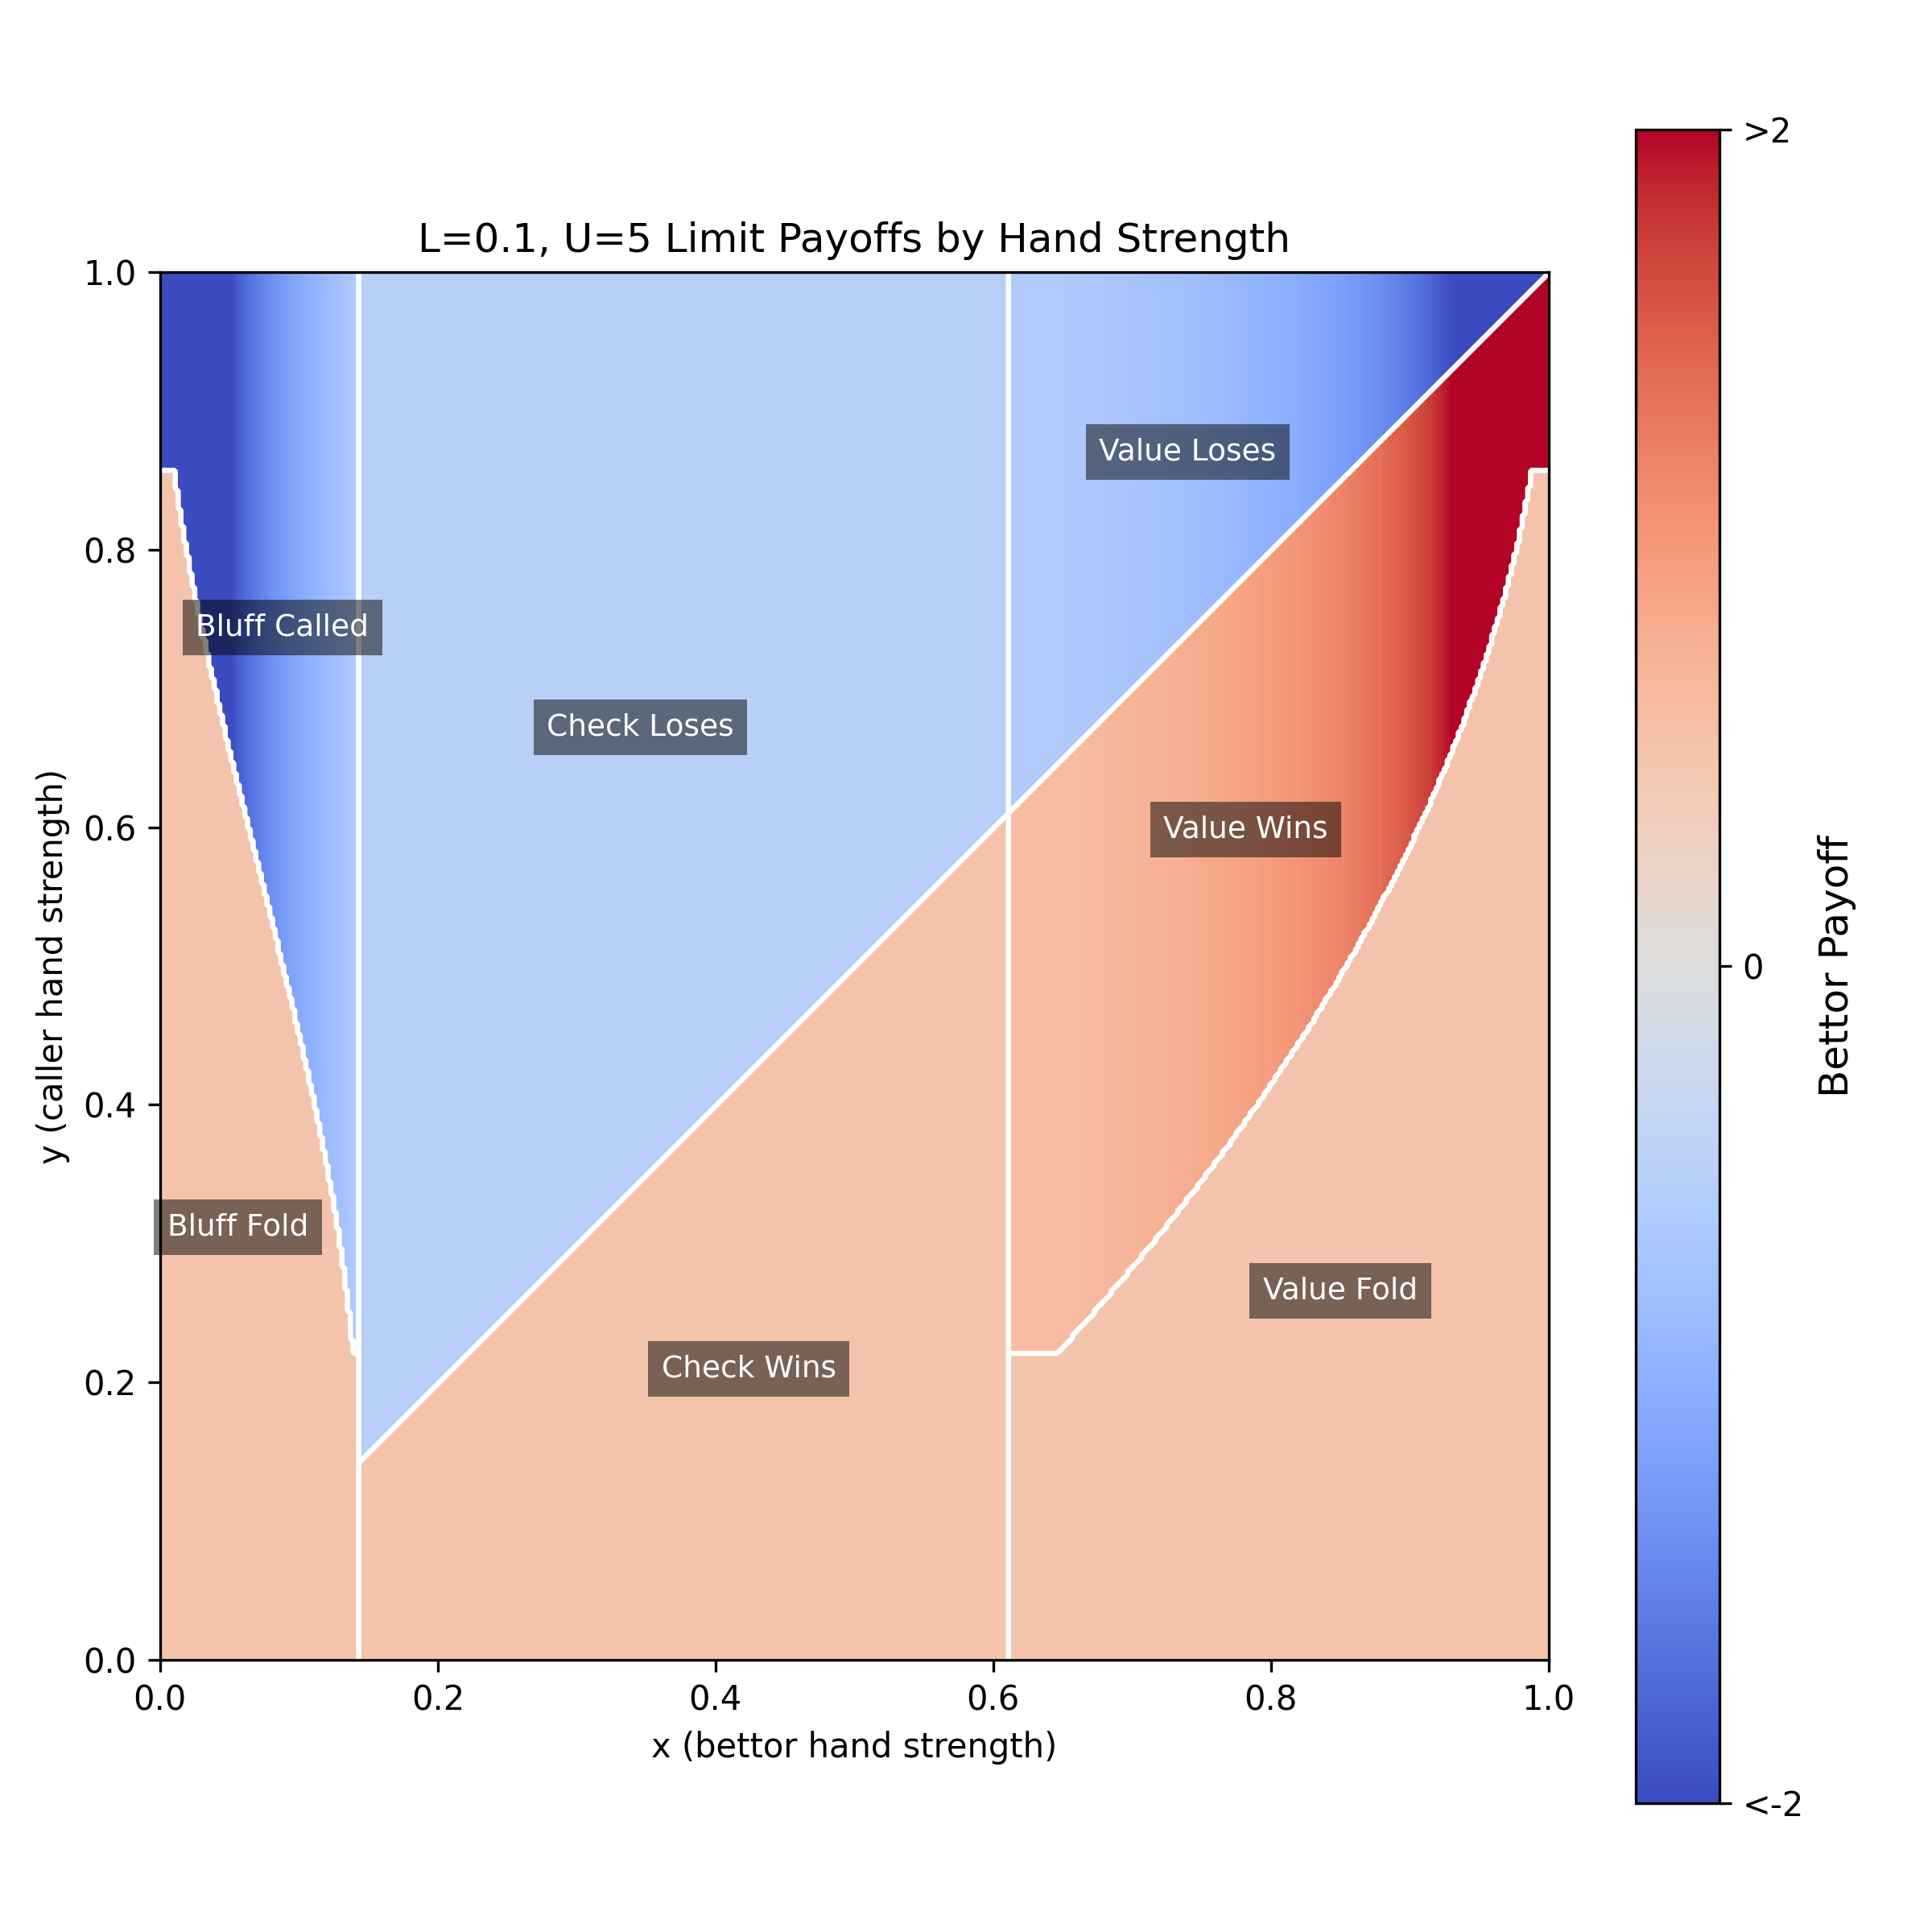
\includegraphics[width=\textwidth]{LU_payoffs_0.1_5.png}
        \end{minipage}
        \hspace{0.02\textwidth}
        \begin{minipage}{0.4\textwidth}
            \centering
            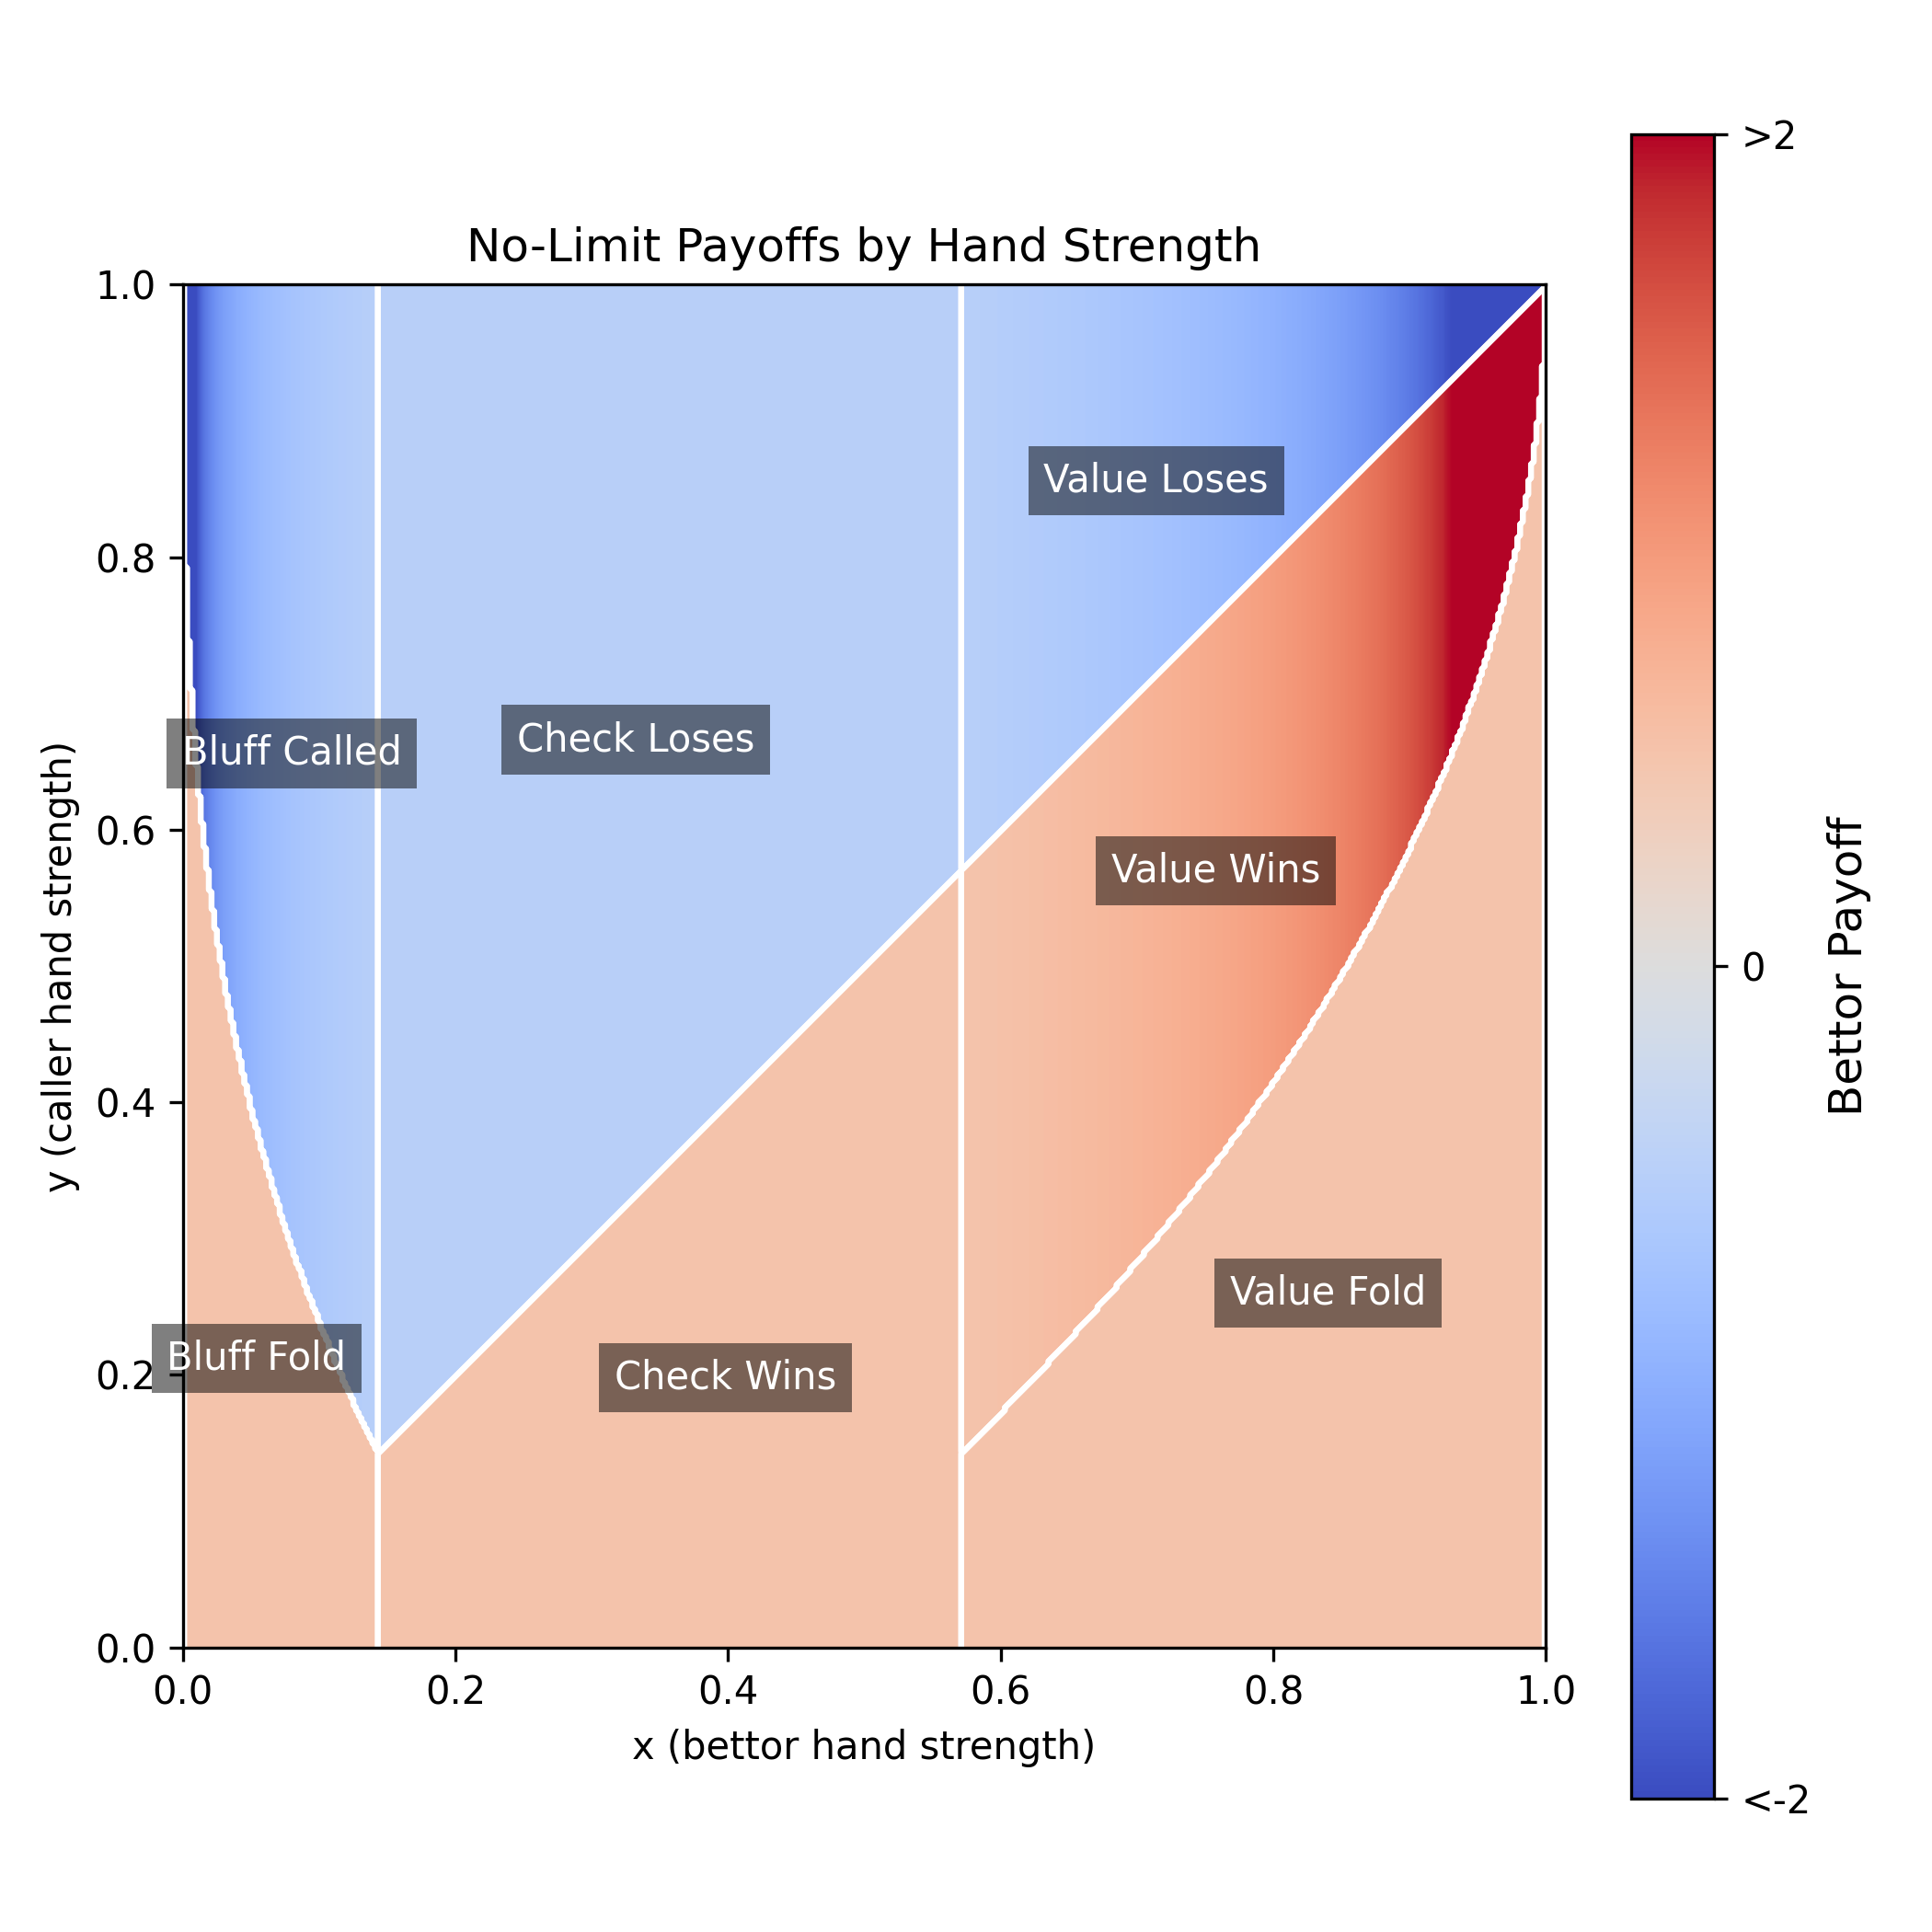
\includegraphics[width=\textwidth]{payoff_heatmap_with_regions_labeled.png}
        \end{minipage}
    \end{adjustwidth}
    \caption{Bettor payoffs in Nash equilibrium as a function of hand strengths $x, y$, for different values of $L$ and $U$ ranging from strict (fixed bet size $B=1$) to lenient (No limits). Regions are labeled according to the outcome of the game in Nash equilibrium.}
    \label{fig:payoffs}
\end{figure}

We saw earlier how the most extreme payoffs occur when the caller has a strong hand and the bettor has either a very strong or very weak hand. As the limits become more lenient, these cases become more extreme but also less likely, since making and calling maximum bets become more risky for both players. 

It is worth noting that the bettors strongest hands (right edge) actually become less likely to make any profit as limits increase. These strongest hands make very large bets, which force all but the strongest hands to fold, but win huge pots when they do get called. In more complicated poker variants, it is common to `slowplay' strong hands by checking or making small bets to induce bluffs from the opponent. In LCP, the inability of the caller to raise makes slowplaying obsolete; with extremely strong hands, forcing a bigger pot outweighs the lower likelihood of getting called.

We also observe that as the limits become more lenient, the checking region shrinks. This is because the bettor can make use of small bets for hands that might have otherwise checked. 

% \begin{figure}[h!]
%     \centering
%     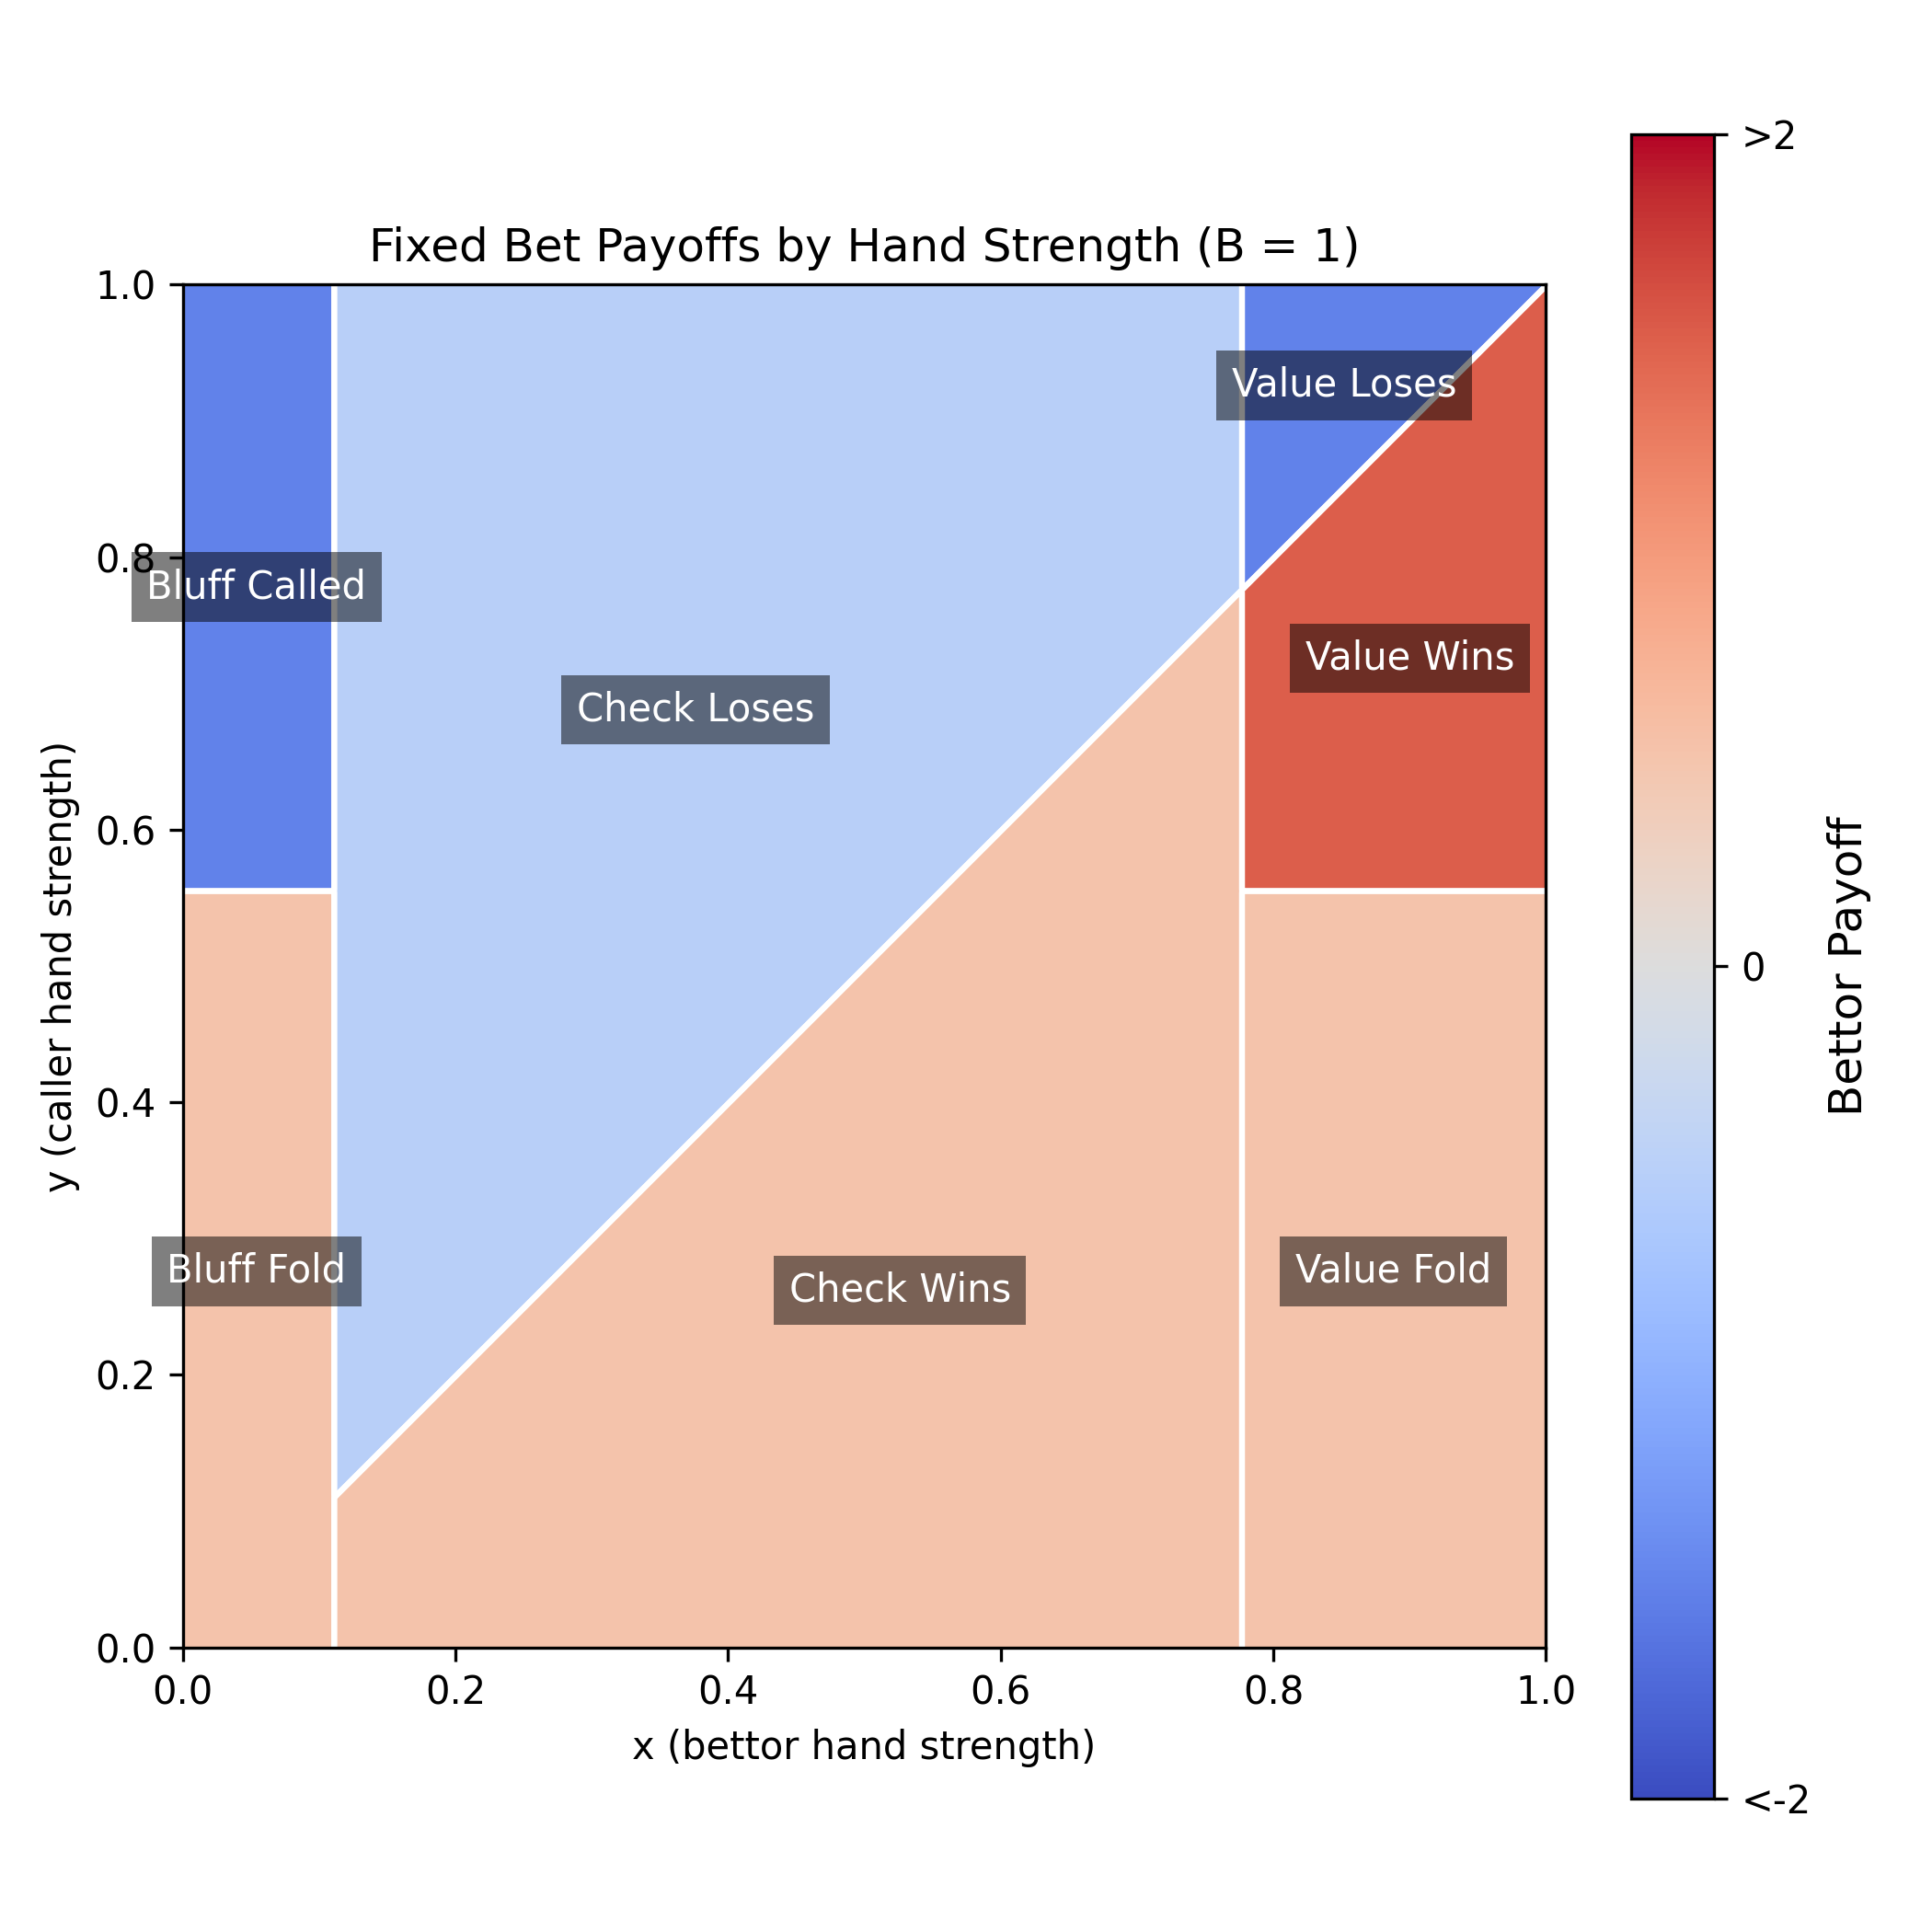
\includegraphics[width=0.7\textwidth]{payoff_fixed_bet_heatmap.png}
%     \caption{Nash equilibrium payoffs for Continuous Poker for all possible hand strength combinations, with fixed bet size $B=1$.}
%     \label{fig:payoff}
% \end{figure}
% \todo{comparison with Limit Continuous Poker for limits close to eachother}






% \begin{figure}[h!]
%     \centering
%     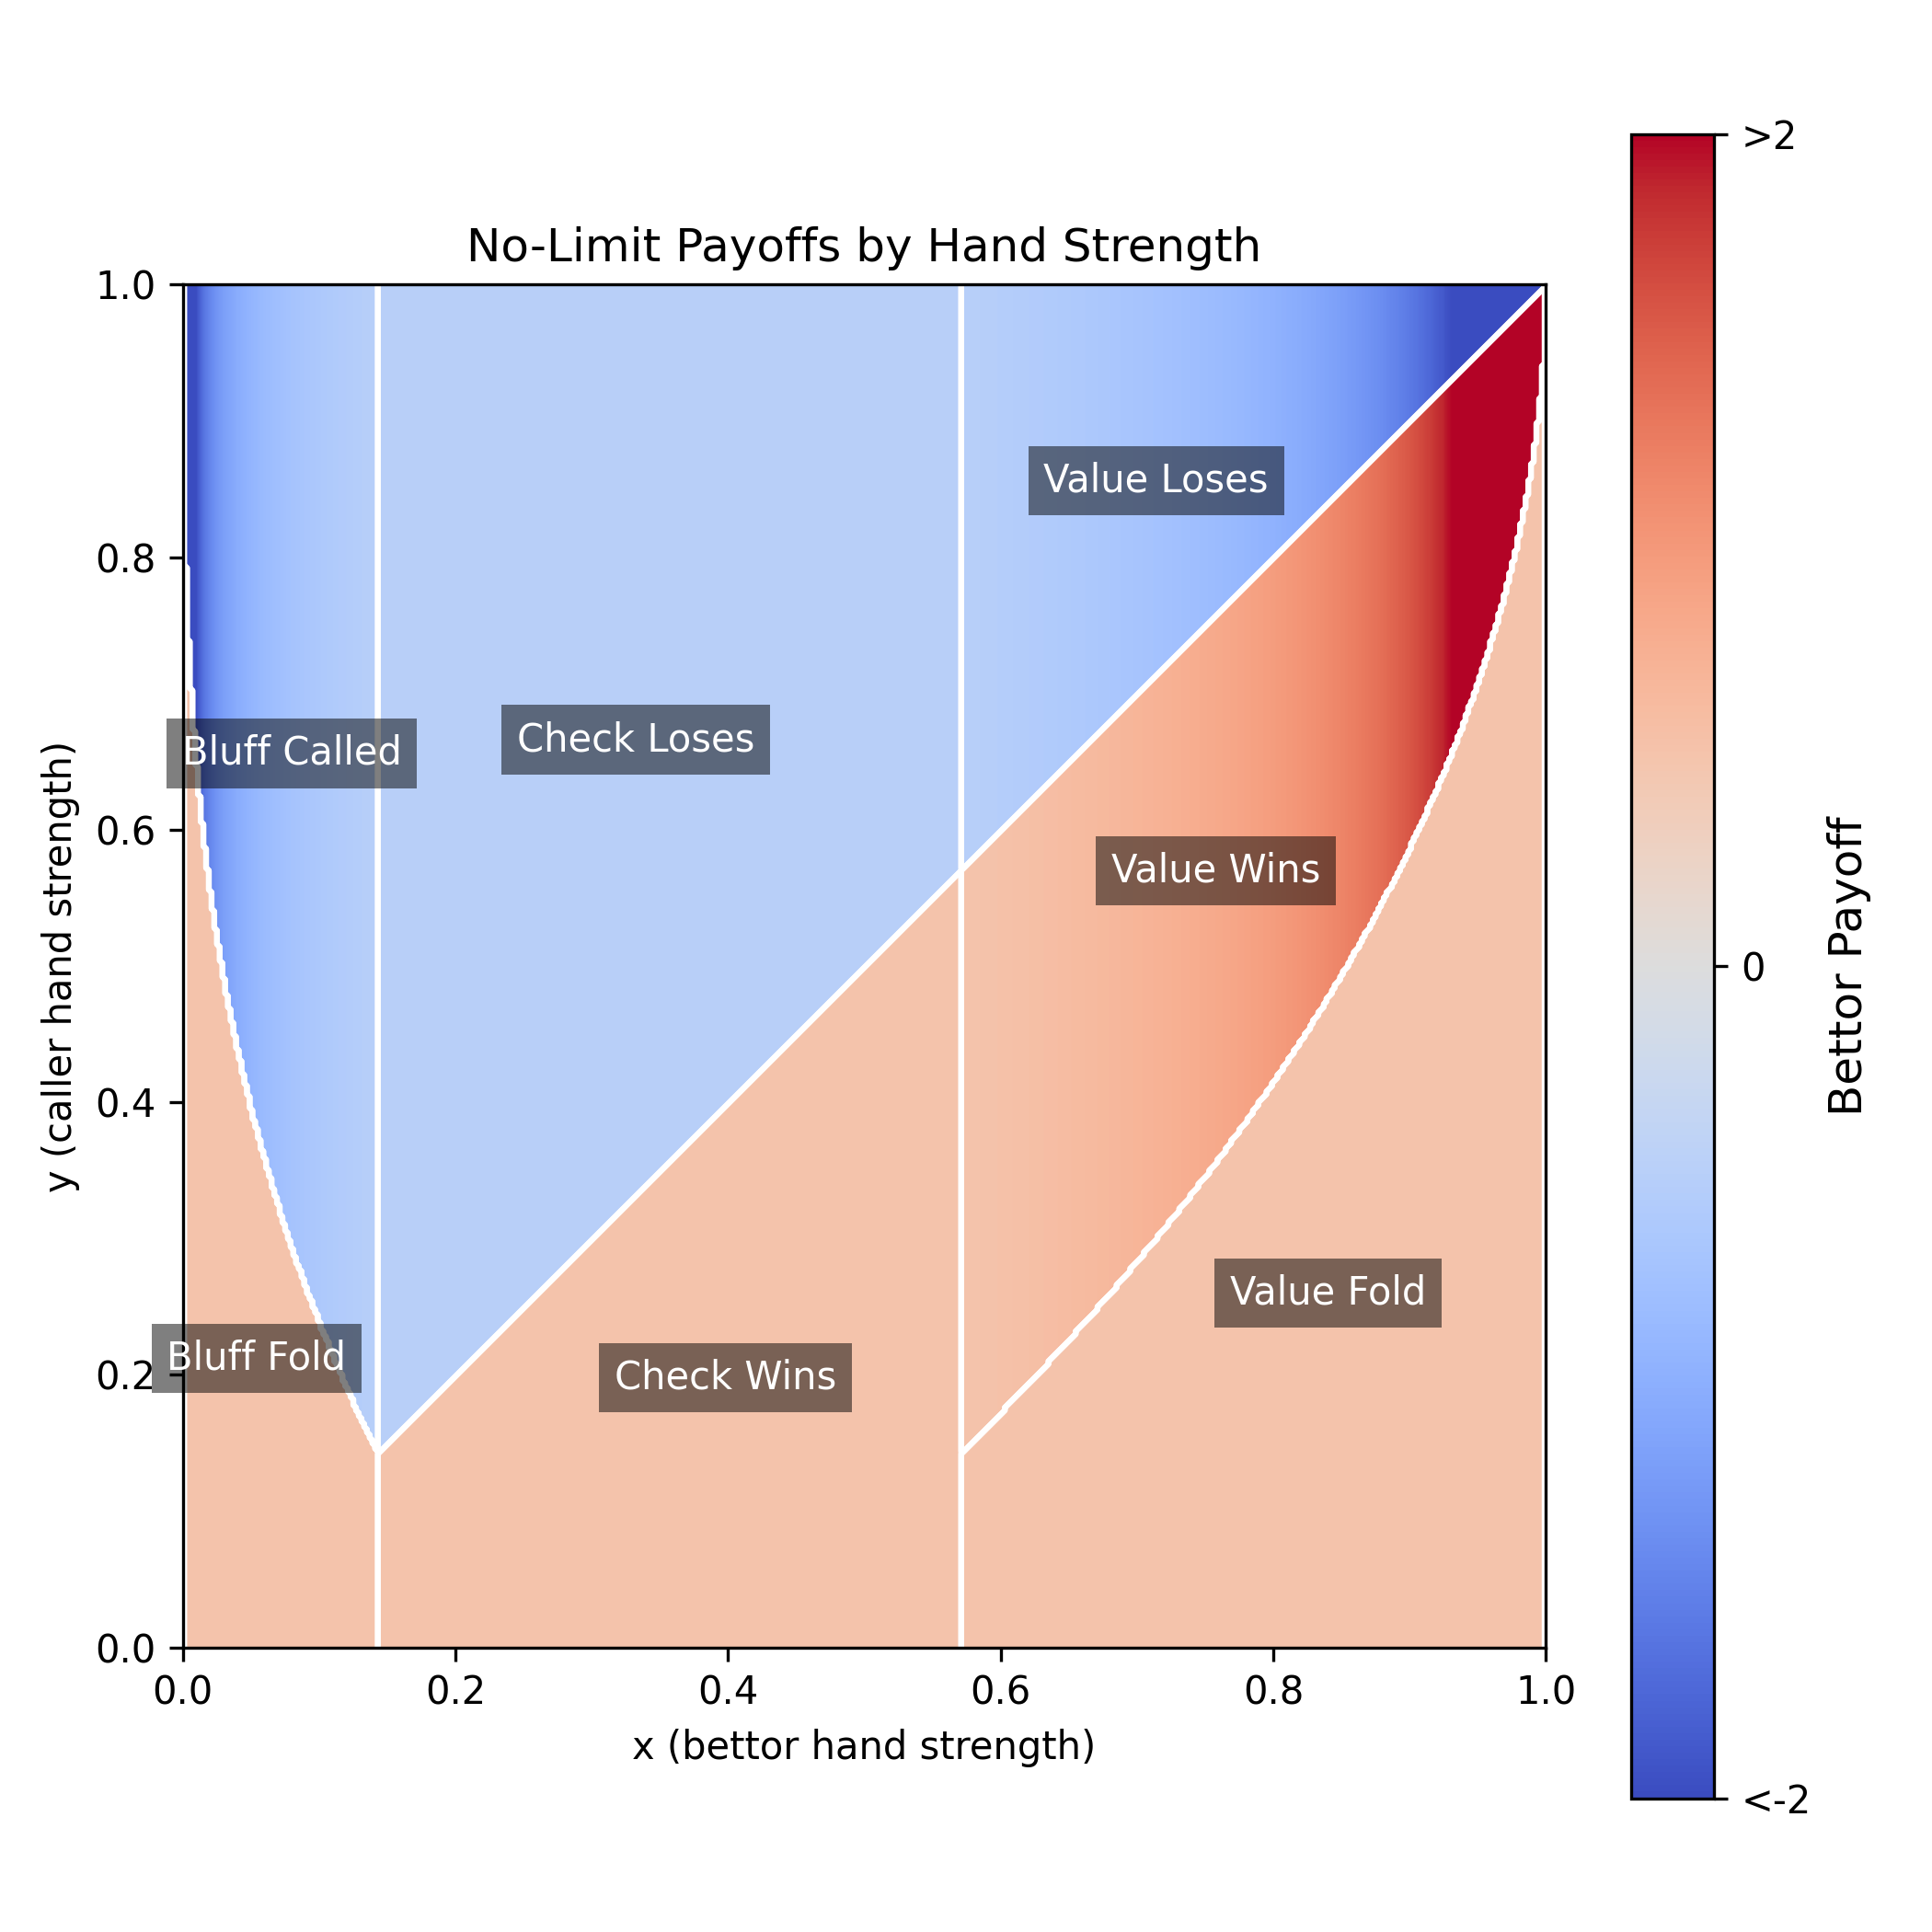
\includegraphics[width=0.7\textwidth]{payoff_heatmap_with_regions_labeled.png}
%     \caption{Nash equilibrium payoffs for NLCP for all possible hand strength combinations.}
%     \label{fig:no-limit-payoff}
% \end{figure}
% \todo{comapre with limit FBCP for lenient limits}



\end{document}
